\chapter{电磁场的基本定律}
电磁学的三大基本定律(库伦定律、安培力定律、法拉第电磁感应定律)的提出,标志着人类对宏观电磁现象的认识从定性阶段到定量阶段的飞跃。以三大实验定律为基础,麦克斯韦提出了两个基本假设(涡旋电场假设、位移电流假设),进而归纳出总结出描述宏观电磁现象的基本定律,麦克斯韦方程组。麦克斯韦方程组的建立,是对电磁理论进步的重大贡献,以麦克斯韦方程组为核心的宏观电磁理论,是研究电磁现象和解决现代工程电磁问题的理论基础。

在本章中,首席将介绍产生电磁场的源,即电荷和电流,再从实验定律引入描述电磁场的基本物理量,即电场强度$\vb*{E}$和磁感强度$\vb*{B}$,并讨论其散度特性和旋度特性。接着讨论介质的电磁特性,然后讨论涡旋电场和位移电流,最后,引出麦克斯韦方程组并讨论电磁场的边界条件。

\section{电荷守恒与电流连续性}
电荷周围要产生电场,电流周围要产生磁场,电荷电流是产生电磁场的源量。

\subsection{电荷与电荷密度}
自然界中存在两种\uwave{电荷}(Electric Charge):\uwave{正电荷}和\uwave{负电荷}。带电体所带电量称为\uwave{电荷量},电荷量并非是连续变化的,电荷量只能取值基本电荷$e=1.602\times 10^{-19}\si{C}$的整数倍,即,电荷是以离散方式分布的。基本电荷$e$恰好就是质子和电子的电荷量,质子带电$e$,电子带电$-e$。

电荷通常以$q$表示,尽管我们说,电荷实际上是离散分布的,但在研究宏观电磁现象时,我们所观察到的是带电体上大量微观带电粒子的总体效应,而带电粒子的线度又远小于带电体的线度。因此,我们可以近似认为,电荷是连续分布在带电体上的,并可以用电荷密度来描述。

\begin{BoxDefinition}[电荷体密度]*
    连续分布在体积$V$内的电荷,称为\uwave{体分布电荷}或\uwave{体电荷}(Volume Charge)。

    体电荷的分布,用\uwave{电荷体密度}(Volume Charge Density)表示
    \begin{Equation}
        \rho(\vb*{r},t)=\Lim[\delt{V}\to 0]\frac{\delt{q}(\vb*{r},t)}{\delt{V}}=\dv{q(\vb*{r},t)}{V}
    \end{Equation}
    体积$V$内的电荷量可以用电荷体密度$\rho(\vb*{r},t)$在$V$内的积分求出
    \begin{Equation}
        q(t)=\Itnt[V]\rho(\vb*{r},t)\dd{V}
    \end{Equation}
\end{BoxDefinition}

除了电荷体密度,亦有适用于面分布的面密度和线分布的线密度。

\begin{BoxDefinition}[电荷面密度]
    连续分布在曲面$S$内的电荷,称为\uwave{面分布电荷}或\uwave{面电荷}(Surface Charge)。

    面电荷的分布,用\uwave{电荷面密度}(Surface Charge Density)表示
    \begin{Equation}
        \rho_S(\vb*{r},t)=\Lim[\delt{S}\to 0]\frac{\delt{q}(\vb*{r},t)}{\delt{S}}=\dv{q(\vb*{r},t)}{S}
    \end{Equation}
    曲面$S$内的电荷量可以用电荷面密度$\rho_S(\vb*{r},t)$在$V$内的积分求出
    \begin{Equation}
        q(t)=\Isnt[S]\rho_S(\vb*{r},t)\dd{S}
    \end{Equation}
\end{BoxDefinition}

\begin{BoxDefinition}[电荷线密度]
    连续分布在曲线$l$内的电荷,称为\uwave{线分布电荷}或\uwave{线电荷}(Linear Charge)。

    线电荷的分布,用\uwave{电荷线密度}(Linear Charge Density)表示
    \begin{Equation}
        \rho_l(\vb*{r},t)=\Lim[\delt{l}\to 0]\frac{\delt{q}(\vb*{r},t)}{\delt{l}}=\dv{q(\vb*{r},t)}{l}
    \end{Equation}
    曲线$l$内的电荷量可以用电荷线密度$\rho_l(\vb*{r},t)$在$l$内的积分求出
    \begin{Equation}
        q(t)=\Int[l]\rho_l(\vb*{r},t)\dd{l}
    \end{Equation}
\end{BoxDefinition}

当带电体的线度,远小于观察点至带电体的距离时,此时,带电体的形状和电荷分布以及无关紧要,带电体可以近似为一个电荷集中在中心的几何点模型,称为\uwave{点电荷}(Point Charge)。

点电荷的概念在电磁理论中有很重要的地位,就像质点与之经典力学那般。

点电荷是电荷分布的一种极限情况,点电荷可以视为一个体积很小而带电量一定的带电球体在半径$a\to 0$时的极限。设电荷$q(t)$分布在位于$\vb*{r}'$半径为$a$的球体内,那么
\begin{itemize}
    \item 在$|\vb*{r}-\vb*{r}'|>a$的球外区域,电荷密度显然为零。
    \item 在$|\vb*{r}-\vb*{r}'|<a$的球内区域,电荷密度将为非常大的数值(由于球体很小),当$a\to 0$时球心$\vb*{r}=\vb*{r'}$处的电荷密度将趋于无穷大,而$\vb*{r}\neq\vb*{r}'$处的电荷密度则均为零,但整个极限过程中,电荷总量保持为$q(t)$不变。这也就是说,电荷密度$\rho(\vb*{r},t)$在全空间的积分是定值,在$\vb*{r}=\vb*{r}'$为无穷大,在$\vb*{r}\neq\vb*{r}'$为零,这在数学上完全符合狄拉克函数的特性。
\end{itemize}
因此,点电荷的电荷密度可以用狄拉克函数描述。
\begin{BoxDefinition}[点电荷]
    点电荷的电荷密度可以用狄拉克函数描述
    \begin{Equation}
        \rho(\vb*{r},t)=q(t)\dirac(\vb*{r}-\vb*{r}')
    \end{Equation}
    其中,$q(t)$是点电荷的电荷量,$\vb*{r}'$是点电荷的位矢。
\end{BoxDefinition}

\subsection{电流与电流密度}\vspace{-0.25cm}
\begin{BoxDefinition}[电流]
    \uwave{电流}(Electric Current)是由电荷运动形成的,定义为
    \begin{Equation}
        i(t)=\Lim[\delt{t}\to 0]\frac{\delt{q}(t)}{\delt{t}}=\dv{q(t)}{t}
    \end{Equation}
    其中,$\delt{q}(t)$表示在$\delt{t}$的时间内通过某一曲面$S$的电荷量,$i(t)$即通过曲面$S$的电流。
\end{BoxDefinition}

电流的意义是单位时间通过某一曲面$S$的电荷量,因此,我们不能说某一点的电流是多少,但是,我们又迫切的需要了解电流的分布情况,介于不同点处的电荷运动方向往往是不同的。

电流密度$\vb*{J}(\vb*{r},t)$就是为此而引入的,在$\vb*{r}$处的电流密度是如何计算的呢?我们在$\vb*{r}$处垂直电荷运动的方向上取一个面积元$\delt{S}$,其法向单位矢量为$\vb*{e}_\text{n}$,电流密度的大小即该面积元上的电流$\delt{i}$与该面积元$\delt{S}$的比在$\delt{S}\to 0$的极限,电流密度的方向就是该处$\vb*{e}_\text{n}$的方向。

\begin{BoxDefinition}[电流密度]
    \uwave{电流密度}(Current Density)描述了电流的分布
    \begin{Equation}
        \vb*{J}(\vb*{r},t)=\vb*{e}_\text{n}\Lim[\delt{S}\to 0]\frac{\delt{i}(\vb*{r})}{\delt{S}}=\vb*{e}_\text{n}\dv{i(\vb*{r})}{S}
    \end{Equation}
    电流则是电流密度的通量,通过曲面$S$的电流可以被表示为
    \begin{Equation}
        i(t)=\Isnt[S]\vb*{J}(\vb*{r},t)\cdot\dd{\vb*{S}}
    \end{Equation}
\end{BoxDefinition}
\begin{BoxFormula}[电流密度与电荷密度]
    电流密度,是电荷密度与电荷运动速度的乘积
    \begin{Equation}
        \vb*{J}(\vb*{r},t)=\rho\vb*{v}
    \end{Equation}
\end{BoxFormula}\nopagebreak

上述的电流体密度$\vb*{J}(\vb*{r},t)$描述的是体分布电流,我们还可以定义电流面密度$\vb*{J}_S(\vb*{r},t)$来描述面分布电流。但是,我们没有“电流线密度”的概念,因为“电流线密度”就是“电流$i$”,这种线电流的模型是很常用的,例如导线的横截面相较其长度而言很小,就可以视为线电流。\goodbreak

在分析电磁场时,常会使用\uwave{电流元}(Current Element)的概念,对于线电流,我们会沿电流流动方向取一个线元矢量$\dd{\vb*{l}}$,并将$i\dd{\vb*{l}}$称为电流元。而对于体分布电流和面分布电流,其电流元分别是$\vb*{J}\dd{V}$和$\vb*{J}_S\dd{S}$。在某种意义上,载流导体可以视为由电流元“积分”而来的。


\subsection{电荷守恒定律与电流连续性方程}
电荷是守恒的,它既不能被创造,也不能被消灭,只能从物体的一个部分转移到另一部分,或者从一个物体转移到另一个物体,这就是所谓\uwave{电荷守恒定律}(Law of Charge Conservation)。

电荷守恒定律的直接结果,就是\uwave{电流连续性方程}(Continuity Equation)。

\begin{BoxEquation}[电流连续性方程]
    电流连续性方程是指,电流场$\vb*{J}(\vb*{r},t)$满足以下方程
    \begin{Equation}
        \div\vb*{J}+\pdv{\rho}{t}=0
    \end{Equation}
    特别的,对于恒定电流场
    \begin{Equation}
        \div{\vb*{J}}=0
    \end{Equation}
\end{BoxEquation}
\begin{Proof}
    任取一个边界曲面为$S$的空间区域$V$,应有
    \begin{Equation}&[1]
        \Isot[S]{\vb*{J}\cdot\dd{\vb*{S}}}=-\dv{q}{t}=-\dv{t}\Itnt[V]\rho\dd{V}
    \end{Equation}
    这是因为,\xrefpeq{1}左端代表的是单位时间内从$S$流出的电荷,\xrefpeq{1}右端代表的是单位时间在空间区域$V$内减少的电荷,根据前述的电荷守恒定律,这两者很明显应该是相等的。

    由于$V$不会随时间变化,不妨将\xrefpeq{1}右端对时间的求导置于积分内
    \begin{Equation}&[2]
        \Isot[S]\vb*{J}\cdot\dd{\vb*{S}}=-\Itnt[V]\pdv{\rho}{t}\dd{V}
    \end{Equation}
    就\xrefpeq{2}的左端运用\fancyref{thm:散度定理}
    \begin{Equation}
        \Itnt[V]\div\vb*{J}\dd{V}=-\Itnt[V]\pdv{\rho}{t}\dd{V}
    \end{Equation}
    即
    \begin{Equation}
        \Itnt[V]\qty(\div\vb*{J}+\pdv{\rho}{t})\dd{V}=0
    \end{Equation}
    由于$V$是任取的
    \begin{Equation}
        \div\vb*{J}+\pdv{\rho}{t}=0
    \end{Equation}
    而恒定电流场中,电荷分布$\rho$不随时间变化,因此$\pdv*{\rho}{t}=0$。
\end{Proof}
电流连续性方程指出,\empx{时变电流场是有散场}
\begin{itemize}
    \item 电流场在电荷密度随时间减少的地方,发出电流线,构成电流场的源。
    \item 电流场在电荷密度随时间增加的地方,终止电流线,构成电流场的汇。
\end{itemize}
恒定电流场的电荷密度不随时间变化,因此没有源或汇,换言之,\empx{恒定电流场是无散场}。


\section{真空中静电场的基本规律}

电荷周围的空间存在电场,电场对电荷会产生作用力,称为电场力,这就是电场的基本特征。

\subsection{电场的基本特征}
\begin{BoxLaw}[电场的基本特性]
    若电场中存在电荷$q$,则其所受到的电场力,具有以下特性
    \begin{Equation}
        \vb*{F}_\text{c}=q\vb*{E}
    \end{Equation}
    其中$\vb*{E}$称为\uwave{电场强度}(Electric Field Intensity),单位是$\si{V\cdot m^{-1}}$。
\end{BoxLaw}

\subsection{电场的基本实验定律}
在1785年,法国科学家库伦(Coulomb)通过著名的“扭秤实验”,总结出真空中两个静止电荷$q_1$和$q_2$间的相互作用力的规律,称为\uwave{库伦定律}(Coulomb's Law),这是电场的基本实验定律,因此电场力也被称为\uwave{库伦力}(Coulomb Force)。库伦定律的内容可以叙述如下
\begin{BoxLaw}[库伦定律]
    设点电荷$q_1$和$q_2$的位矢分别为$\vb*{r}_1$和$\vb*{r}_2$,记$\vb*{R}_{12}=\vb*{r}_2-\vb*{r}_1$是$q_1$指向$q_2$的矢量。

    那么,$q_1$在$q_2$上产生的作用力$\vb*{F}_{12}$为
    \begin{Equation}
        \vb*{F}_{12}=\frac{q_1q_2}{4\pi\varepsilon_0R_{12}^3}\vb*{R}_{12}
    \end{Equation}
    其中物理常数$\varepsilon_0$被称为\uwave{真空电容率}(Vacuum Permittivity)\footnote[2]{除了真空电容率,有时$\varepsilon_0$也被称为真空介电常数。},其值为
    \begin{Equation}
        \varepsilon_0=(1/36\pi)\times 10^{-9}\si{F\cdot m^{-1}}
    \end{Equation}
\end{BoxLaw}

库伦定律指出,电荷间的作用满足平方反比关系,同号电荷相互排斥,异号电荷相互吸引。

库伦定律讨论的是两个电荷间的相互作用,设真空中有$N$个点电荷$q_1,q_2,\cdots,q_N$分别位于位矢$\vb*{r}_1',\vb*{r}_2',\cdots,\vb*{r}_N'$处,它们将作为电场的源点。那么,位于场点$\vb*{r}$处的点电荷$q$所受到的库伦力$\vb*{F}$,就可以依照力的叠加原理,视为$q,q_1$、$q,q_2$、$\cdots$、$q,q_N$两两之间的库伦力的和
\begin{Equation}
    \vb*{F}=\Sum[i=1][N]\frac{qq_iR_i}{4\pi\varepsilon_0R_i^3}=\frac{q}{4\pi\varepsilon_0}\Sum[i=1][N]\frac{q_i\vb*{R}_i}{R_i^3}
\end{Equation}
其中$\vb*{R}_i=\vb*{r}-\vb*{r}_i$,即由场点指向各个源点的矢量。

而根据\fancyref{law:电场的基本特性},我们很容易得出测试点电荷$q$处的电场强度应为
\begin{Equation}
    \vb*{E}(\vb*{r})=\frac{1}{4\pi\varepsilon_0}\Sum[i=1][N]\frac{q_i\vb*{R}_i}{R_i^3}
\end{Equation}
而对于连续带电体,上式将转化为积分
\begin{BoxFormula}[电场强度]
    电场强度$\vb*{E}(\vb*{r})$符合以下规律
    \begin{Equation}
        \vb*{E}(\vb*{r})=\frac{1}{4\pi\varepsilon_0}\Itnt[V]\frac{\rho(\vb*{r}')\vb*{R}}{R^3}\dd{V'}
    \end{Equation}
    其中$\vb*{R}=\vb*{r}-\vb*{r}'$,而$\rho(\vb*{r}')$则给出$V$中源点$\vb*{r}'$处的电荷密度。
\end{BoxFormula}

\subsection{距离反比的拉普拉斯}
在开始讨论静电场的性质之前,我们先需要补充一个重要的数学公式。\cite{W2}
\begin{BoxFormula}[距离反比的拉普拉斯]
    设位矢$\vb*{r}$,$r=\abs{\vb*{r}}$,则有
    \begin{Equation}
        \laplacian(\frac{1}{r})=-4\pi\dirac(\vb*{r})
    \end{Equation}
    若记$\vb*{R}=\vb*{r}-\vb*{r}'$,$\vb*{r}$为场点,$\vb*{r}'$为源点常量,则有
    \begin{Equation}
        \laplacian(\frac{1}{R})=-4\pi\dirac(\vb*{R})=-4\pi\dirac(\vb*{r}-\vb*{r}')
    \end{Equation}
\end{BoxFormula}
\begin{Proof}
    根据\fancyref{fml:球坐标系的拉普拉斯},若$r\neq 0$
    \begin{Equation}
        \laplacian(\frac{1}{r})=\frac{1}{r^2}\pdv{r}\qty[r^2\pdv{(1/r)}{r}]=\frac{1}{r^2}\pdv{r}\qty[r^2\qty(-\frac{1}{r^2})]=0
    \end{Equation}
    而若$r\neq 0$,上式不再适用,我们试着对$\laplacian(1/r)$在$V$上积分
    \begin{Equation}
        \qquad\qquad\qquad
        I=\Itnt[V]\laplacian(\frac{1}{r})\dd{V}=\Itnt[V_0]\laplacian(\frac{1}{r})\dd{V}+\Itnt[V-V_{0}]\laplacian(\frac{1}{r})\dd{V}
        \qquad\qquad\qquad
    \end{Equation}
    这里将$V$拆分为两部分,$V_0$是以原点为球心,半径为$r_0$的球形区域,半径$r_0$可以任取以确保$V_0$完全在$V$之内。而$V-V_0$是剩余区域,由于$V-V_0$不包含原点,因此其积分为零。

    因此,在$V$上的积分就可以转化为球形区域$V_0$上的积分
    \begin{Equation}
        I=\Itnt[V]\laplacian(\frac{1}{r})\dd{V}=
        \Itnt[V_0]\laplacian(\frac{1}{r})\dd{V}
    \end{Equation}
    运用\fancyref{thm:散度定理}
    \begin{Equation}
        I=
        \Itnt[V_0]\div\grad(\frac{1}{r})\dd{V}=
        \Isot[S_0]\grad(\frac{1}{r})\cdot\dd{\vb*{S}}
    \end{Equation}
    其中$S_0$为$V_0$的边界曲面,即半径为$r_0$的球面,而球面上的积分是可以计算的
    \begin{Equation}
        I=\Isot[S_0]\grad(\frac{1}{r})\cdot\frac{\vb*{r}_0}{r_0}\dd{S}=\Int[0][2\pi]\Int[0][\pi]\grad(\frac{1}{r})\cdot\frac{\vb*{r}_0}{r_0}r_0^2\sin\theta\dd{\theta}\dd\phi
    \end{Equation}
    代入\fancyref{fml:距离反比的梯度},注意到$r_0$被完全约去
    \begin{Equation}
        \qquad\qquad
        I=\Int[0][2\pi]\Int[0][\pi]-\frac{\vb*{r}_0}{r_0^3}\cdot\frac{\vb*{r}_0}{r_0}r_0^2\sin\theta\dd{\theta}\dd\phi=\Int[0][2\pi]\Int[0][\pi]-\sin\theta\dd{\theta}\dd\phi=-4\pi
        \qquad\qquad
    \end{Equation}
    在这里,我们看到,$\laplacian(1/r)$在$r\neq 0$时处处为零,但是,$\laplacian(1/r)$在包含$r=0$的空间上的积分却并不是零,而是有限值$-4\pi$,这就意味着$\laplacian(1/r)$需要用狄拉克函数表示,即
    \begin{Equation}*
        \laplacian(\frac{1}{r})=-4\pi\dirac(\vb*{r})\qedhere
    \end{Equation}
\end{Proof}\vspace{-0.25cm}

\subsection{静电场的散度}
\begin{BoxProperty}[静电场的散度]*
    静电场的散度满足
    \begin{Equation}
        \div\vb*{E}=\frac{\rho}{\varepsilon_0}
    \end{Equation}
    该性质也可以改写为积分形式
    \begin{Equation}
        \Isot[S]\vb*{E}\cdot\dd{\vb*{S}}=\frac{1}{\varepsilon_0}\Itnt[V]\rho\dd{V}=\frac{q}{\varepsilon_0}
    \end{Equation}
    该结论称为\uwave{高斯定律}(Gauss's Law)。

    该式表明,电场强度$\vb*{E}$在闭曲面上的通量等于闭曲面内的总电荷与$\varepsilon_0$之比。
\end{BoxProperty}

\begin{Proof}
    根据\fancyref{fml:电场强度}
    \begin{Equation}&[1]
        \vb*{E}(\vb*{r})=\frac{1}{4\pi\varepsilon_0}\Itnt[V]\frac{\rho(\vb*{r}')\vb*{R}}{R^3}\dd{V'}
    \end{Equation}\goodbreak
    根据\fancyref{fml:距离反比的梯度},$\grad(1/R)=-\vb*{R}/R^3$
    \begin{Equation}&[2]
        \vb*{E}(\vb*{r})=-\frac{1}{4\pi\varepsilon_0}\Itnt[V]\rho(\vb*{r}')\grad(\frac{1}{R})\dd{V'}
    \end{Equation}
    在\xrefpeq{2}两端取散度
    \begin{Equation}&[3]
        \div\vb*{E}(\vb*{r})=\div\qty[-\frac{1}{4\pi\varepsilon_0}\Itnt[V]\rho(\vb*{r}')\grad(\frac{1}{R})\dd{V'}]
    \end{Equation}
    由于微分算符$\grad$是对场点$\vb*{r}$的坐标的微分,而\xrefpeq{3}的积分是对源点$\vb*{r}'$坐标进行,故微分算符$\grad$可与积分运算交换顺序,而$\rho(\vb*{r}')$只与源点$\vb*{r}'$有关,也可以移到微分算符$\grad$之外
    \begin{Equation}
        \div\vb*{E}(\vb*{r})=-\frac{1}{4\pi\varepsilon_0}\Itnt[V]\rho(\vb*{r}')\div\grad(\frac{1}{R})\dd{V'}
    \end{Equation}
    梯度的散度即拉普拉斯算符
    \begin{Equation}
        \div\vb*{E}(\vb*{r})=-\frac{1}{4\pi\varepsilon_0}\Itnt[V]\rho(\vb*{r}')\laplacian(\frac{1}{R})\dd{V'}
    \end{Equation}
    利用\fancyref{fml:距离反比的拉普拉斯},$\laplacian(1/R)=-4\pi\dirac(\vb*{R})=-4\pi\dirac(\vb*{r}-\vb*{r}')$
    \begin{Equation}
        \div\vb*{E}(\vb*{r})=\frac{1}{\varepsilon_0}\Itnt[V]\rho(\vb*{r}')\dirac(\vb*{r}-\vb*{r}')\dd{V'}
    \end{Equation}
    利用狄拉克函数的筛选性质
    \begin{Equation}*
        \div\vb*{E}=\frac{\rho}{\varepsilon_0}\qedhere
    \end{Equation}
\end{Proof}

\subsection{静电场的旋度}
\begin{BoxProperty}[静电场的旋度]
    静电场的旋度满足
    \begin{Equation}
        \curl\vb*{E}=\vb*{0}
    \end{Equation}
    该性质也可以改写为积分形式
    \begin{Equation}
        \Ilot[C]\vb*{E}\cdot\dd{\vb*{l}}=0
    \end{Equation}
    该式表明,电场强度$\vb*{E}$在闭曲线上的环流等于零,即,静电场是无旋场。
\end{BoxProperty}
\begin{Proof}
    我们回到静电场散度中的\xrefpeq[静电场的散度]{2}
    \begin{Equation}&[1]
        \vb*{E}(\vb*{r})=-\frac{1}{4\pi\varepsilon_0}\Itnt[V]\rho(\vb*{r}')\grad(\frac{1}{R})\dd{V'}
    \end{Equation}
    由于积分是关于源点$\vb*{r}'$,而微分算符关于常点$\vb*{r}$,故微分算符可以提至积分外
    \begin{Equation}&[2]
        \vb*{E}(\vb*{r})=-\grad[\frac{1}{4\pi\varepsilon_0}\Itnt[V]\frac{\rho(\vb*{r'})}{R}\dd{V'}]
    \end{Equation}
    在\xrefpeq{2}两端取旋度
    \begin{Equation}&[3]
        \curl\vb*{E}=-\curl\grad[\frac{1}{4\pi\varepsilon_0}\Itnt[V]\frac{\rho(\vb*{r'})}{R}\dd{V'}]
    \end{Equation}
    在\xrefpeq{3}右端,是一个标量场梯度的旋度,而根据\fancyref{ppt:标量场的梯度无旋}
    \begin{Equation}*
        \curl\vb*{E}=\vb*{0}\qedhere
    \end{Equation}
\end{Proof}
\section{真空中静磁场的基本规律}
电流周围的空间存在磁场,磁场对电流产生作用力,称为磁场力,这就是磁场的基本特征。

\subsection{磁场的基本特征}
\begin{BoxLaw}[磁场的基本特征]
    若磁场中存在速度$\vb*{v}$的电荷$q$,则其所受到的磁场力,具有以下特性
    \begin{Equation}
        \vb*{F}_\text{m}=q\vb*{v}\times\vb*{B}
    \end{Equation}
    其中$\vb*{B}$称为\uwave{磁场强度}(Magnetic Induction Intensity),单位是$\si{T}$或$\si{Wb. m^{-2}}$。
\end{BoxLaw}
我们通常将运动电荷受到的磁场力称为\uwave{洛伦兹力}(Lorentz Force)。\footnote{有时洛伦兹力亦指运动电荷受到的电场力和磁场力的总和,即$\vb*{F}=q(\vb*{E}+\vb*{v}\times\vb*{B})$。}

\subsection{磁场的基本实验定律}
在1820年,法国科学家安培(Ampere)通过实验,总结出真空中两电流回路$C_1$和$C_2$之间相互作用力的规律,称为\uwave{安培力定律}(Ampere's Force Law)。这是磁场的基本实验定律。

\begin{BoxLaw}[安培力定律]*
    设分别载有恒定电流$I_1,I_2$的载流细导线回路$C_1,C_2$,记两者的电流元$I_1\dd{\vb*{l}_1},I_2\dd{\vb*{l}_2}$的位置矢量分别为$\vb*{r}_1$和$\vb*{r}_2$,记$\vb*{R}_{12}=\vb*{r}_2-\vb*{r}_1$是电流元$I_1\dd{\vb*{l}_1}$指向$I_2\dd{\vb*{l}_2}$的矢量。

    那么,$C_1$在$C_2$上产生的作用力$\vb*{F}_{12}$为
    \begin{Equation}
        \vb*{F}_{12}=\frac{\mu_0}{4\pi}\Ilot[C_2]\Ilot[C_1]\frac{I_2\dd{\vb*{l}_2}\times(I_1\dd{\vb*{l}_1}\times\vb*{R}_{12})}{R_{12}^3}
    \end{Equation}
    或者,$I_1\dd{\vb*{l}_1}$在$I_2\dd{\vb*{l}_2}$上产生的作用力$\dd{\vb*{F}_{12}}$为
    \begin{Equation}
        \dd{\vb*{F}_{12}}=\frac{\mu_0}{4\pi}\frac{I_2\dd{\vb*{l}_2}\times(I_1\dd{\vb*{l}_1}\times\vb*{R}_{12})}{R_{12}^3}
    \end{Equation}
    
    其中物理常数$\mu_0$被称为\uwave{真空磁导率}(Vacuum Permeability),其值为
    \begin{Equation}
        \mu_0=(4\pi)\times 10^{-7}\si{H\cdot m^{-1}}
    \end{Equation}
\end{BoxLaw}

我们通常将电流受到的磁场力称为\uwave{安培力}(Ampere's Force),与电荷的库仑力对应。

我们注意到电流元间的安培力$\dd{\vb*{F}_{12}}$满足
\begin{Equation}
    \dd{\vb*{F}_{12}}=\frac{\mu_0}{4\pi}\frac{I_2\dd{\vb*{l}_2}\times(I_1\dd{\vb*{l}_1}\times\vb*{R}_{12})}{R_{12}^3}
\end{Equation}
而根据\fancyref{law:磁场的基本特征}
\begin{Equation}
    \dd{\vb*{F}_{12}}=I_2\dd{\vb*{l}_2}\times\dd{\vb*{B}_{12}}
\end{Equation}
因此$I_1\dd{\vb*{l}}_1$在$\vb*{r}_2$处产生的磁感强度$\dd{\vb*{B}_{12}}$为
\begin{Equation}
    \dd{\vb*{B}_{12}}=\frac{\mu_0}{4\pi}\frac{I_1\dd{\vb*{l}_1}\times\vb*{R}_{12}}{R_{12}^3}
\end{Equation}
或者改用通常场点和源点的写法
\begin{Equation}[毕奥萨伐尔定律1]
    \dd{\vb*{B}}=\frac{\mu_0}{4\pi}\frac{I\dd{l'}\times\vb*{R}}{R^3}\qquad\vb*{R}=\vb*{r}-\vb*{r}'
\end{Equation}
由此可见,电流元$I\dd{\vb*{l}'}$在场点$\vb*{r}$产生的磁感强度的方向可以由右手螺旋法则确定,即,右手四指由$I\dd{\vb*{l}'}$转向(源点$\vb*{r}'$指向场点$\vb*{r}$的)矢量$\vb*{R}=\vb*{r}-\vb*{r}'$时,右手大拇指所指的方向。

而进一步的,整个回路$C$在场点$\vb*{r}$产生的磁感强度就是
\begin{Equation}[毕奥萨伐尔定律2]
    \vb*{B}(\vb*{r})=\frac{\mu_0}{4\pi}\Ilot[C]\frac{I\dd{\vb*{l}'}\times\vb*{R}}{R^3}
\end{Equation}
这里\xref{eq:毕奥萨伐尔定律1}和\xref{eq:毕奥萨伐尔定律2}均称为\uwave{毕奥--萨法尔定律}(Biot-Savart Law),是1820年毕奥(Biot)和萨伐尔(Savart)根据安培闭合回路相互作用力的实验结果,通过理论上的分析总结出来的。\goodbreak

而对于连续电流分布体,上式的电流元$\vb*{I}\dd{\vb*{l}'}$应用体电流的电流元$\vb*{J}(\vb*{r}')\dd{V}'$代替\nopagebreak
\begin{BoxFormula}[磁感强度]
    磁感强度$\vb*{B}(\vb*{r})$符合以下规律
    \begin{Equation}
        \vb*{B}(\vb*{r})=\frac{\mu_0}{4\pi}\Itnt[V]\frac{\vb*{J}(\vb*{r}')\times\vb*{R}}{R^3}\dd{V'}
    \end{Equation}
    其中$\vb*{R}=\vb*{r}-\vb*{r}'$,而$\vb*{J}(\vb*{r}')$则给出$V$中源点$\vb*{r}'$处的电流密度。
\end{BoxFormula}

\subsection{静磁场的散度}
\begin{BoxProperty}[静磁场的散度]
    静磁场的散度满足
    \begin{Equation}
        \div\vb*{B}=0
    \end{Equation}
    该性质也可以改写为积分形式
    \begin{Equation}
        \Isot[S]\vb*{B}\cdot\dd{\vb*{S}}=0
    \end{Equation}
    该式表明,磁感强度$\vb*{B}$在闭曲面上的通量等于零,即,静磁场是无散场。
\end{BoxProperty}

\begin{Proof}
    根据\fancyref{fml:磁感强度}
    \begin{Equation}&[1]
        \vb*{B}(\vb*{r})=\frac{\mu_0}{4\pi}\Itnt[V]\frac{\vb*{J}(\vb*{r}')\times\vb*{R}}{R^3}\dd{V'}
    \end{Equation}
    根据\fancyref{fml:距离反比的梯度},$\grad(1/R)=-\vb*{R}/R^3$
    \begin{Equation}&[2]
        \vb*{B}(\vb*{r})=-\frac{\mu_0}{4\pi}\Itnt[V]\vb*{J}(\vb*{r}')\times\grad(\frac{1}{R})\dd{V'}
    \end{Equation}
    根据矢量恒等式
    \begin{Equation}&[3]
        \curl(u\vb*{F})=\grad u\times\vb*{F}+u\curl\vb*{F}
    \end{Equation}
    移项
    \begin{Equation}&[4]
        \vb*{F}\times\grad u=u\curl\vb*{F}-\curl(u\vb*{F})
    \end{Equation}
    这里$\vb*{F}$和$u$分别为
    \begin{Equation}&[5]
        \vb*{F}=\vb*{J}(\vb*{r}')\qquad u=\frac{1}{R}
    \end{Equation}
    这样\xrefpeq{5}就可以转化为
    \begin{Equation}&[6]
        \vb*{B}(\vb*{r})=\frac{\mu_0}{4\pi}\Itnt[V]\qty[\curl(\frac{\vb*{J}(\vb*{r}')}{R})-\frac{1}{R}\curl\vb*{J}(\vb*{r}')]\dd{V'}
    \end{Equation}
    此处$\grad$是对场点的微分运算,而$\vb*{J}(\vb*{r}')$是源点的函数,故$\curl\vb*{J}(\vb*{r}')=\vb*{0}$
    \begin{Equation}&[7]
        \vb*{B}(\vb*{r})=\frac{\mu_0}{4\pi}\Itnt[V]\curl\frac{\vb*{J}(\vb*{r}')}{R}\dd{V'}
    \end{Equation}
    此处$\grad$是对场点的微分运算,而积分是关于源点的,故$\grad$可以提出积分外
    \begin{Equation}&[8]
        \vb*{B}(\vb*{r})=\curl\frac{\mu_0}{4\pi}\Itnt[V]\frac{\vb*{J}(\vb*{r}')}{R}\dd{V'}
    \end{Equation}
    在\xrefpeq{8}两端取散度
    \begin{Equation}&[9]
        \div\vb*{B}=\div\qty(\curl\frac{\mu_0}{4\pi}\Itnt[V]\frac{\vb*{J}(\vb*{r}')}{R}\dd{V'})
    \end{Equation}
    在\xrefpeq{9}右端,是一个矢量场旋度的散度,而根据\fancyref{ppt:矢量场的旋度无散}
    \begin{Equation}*
        \div\vb*{B}=0\qedhere
    \end{Equation}
\end{Proof}

\subsection{静磁场的旋度}
\begin{BoxProperty}[静磁场的旋度]
    静磁场的旋度满足
    \begin{Equation}
        \curl\vb*{B}=\mu_0\vb*{J}(\vb*{r})
    \end{Equation}
    该性质也可以改写为积分形式
    \begin{Equation}
        \Ilot[C]\vb*{B}\cdot\dd{\vb*{l}}=\mu_0\Isnt[S]\vb*{J}(\vb*{r})\cdot\dd{\vb*{S}}=\mu_0I
    \end{Equation}
    该结论称为\uwave{安培环路定理}(Ampere's Circuital Law)。

    该式表明,磁感强度$\vb*{B}$在闭曲线上的环流等于闭曲线内的总电流与$\mu_0$之积。
\end{BoxProperty}

\begin{Proof}
    我们回到静磁场散度中的\xrefpeq[静磁场的散度]{8}
    \begin{Equation}&[1]
        \vb*{B}(\vb*{r})=\curl\frac{\mu_0}{4\pi}\Itnt[V]\frac{\vb*{J}(\vb*{r}')}{R}\dd{V'}
    \end{Equation}
    在\xrefpeq{1}两端取旋度
    \begin{Equation}&[2]
        \curl\vb*{B}=\curl\curl\frac{\mu_0}{4\pi}\Itnt[V]\frac{\vb*{J}(\vb*{r}')}{R}\dd{V'}
    \end{Equation}
    这里旋度可以置于积分内
    \begin{Equation}&[3]
        \curl\vb*{B}=\frac{\mu_0}{4\pi}\Itnt[V]\curl\curl\frac{\vb*{J}(\vb*{r}')}{R}\dd{V'}
    \end{Equation}
    根据矢量恒等式
    \begin{Equation}&[4]
        \curl\curl\vb*{F}=\grad(\div\vb*{F})-\laplacian\vb*{F}
    \end{Equation}
    这样\xrefpeq{3}可以转化为
    \begin{Equation}&[5]
        \qquad\qquad
        \curl\vb*{B}=\frac{\mu_0}{4\pi}\grad\Itnt[V]\div\frac{\vb*{J}(\vb*{r}')}{R}\dd{V'}-\frac{\mu_0}{4\pi}\Itnt[V]\laplacian\frac{\vb*{J}(\vb*{r}')}{R}\dd{V'}=I_1-I_2
        \qquad\qquad
    \end{Equation}
    我们先来计算$I_2$,将$\vb*{J}(\vb*{r}')$提出拉普拉斯外,随后应用\fancyref{fml:距离反比的拉普拉斯}
    \begin{Equation}&[6]
        \qquad\qquad
        I_2=\frac{\mu_0}{4\pi}\Itnt[V]\vb*{J}(\vb*{r}')\laplacian\qty(\frac{1}{R})\dd{V'}=-\mu_0\Itnt[V]\vb*{J}(\vb*{r}')\dirac(\vb*{r}-\vb*{r}')\dd{V'}=-\mu_0\vb*{J}(\vb*{r})
        \qquad\qquad
    \end{Equation}
    我们随后计算$I_1$,其难点在于$\div(\vb*{J}(r')/R)$的计算,我们需要将$\grad$转化为$\grad'$。\footnote{我们会问,我们不是已经有\xref{fml:场点坐标和源点坐标的转化}指出$\grad f(\vb*{R})=-\grad' f(\vb*{R})$,这里又在推导什么呢?事实是,\xref{fml:场点坐标和源点坐标的转化}的结论仅限于梯度运算,其只能代表在梯度运算下转换场点坐标和源点坐标相当于一个负号,而散度运算下$\div f(\vb*{R})=-\grad'\cdot f(\vb*{R})$未必成立。}
    \begin{Equation}&[7]
        I_1=\frac{\mu_0}{4\pi}\grad\Itnt[V]\div\frac{\vb*{J}(\vb*{r}')}{R}\dd{V'}
    \end{Equation}

    根据矢量恒等式
    \begin{Equation}&[8]
        \div(u\vb*{F})=\grad u\cdot\vb*{F}+u\div\vb*{F}
    \end{Equation}
    这样$\div(\vb*{J}(\vb*{r}')/R)$就可以展开为
    \begin{Equation}&[9]
        \div\frac{\vb*{J}(\vb*{r}')}{R}=\grad\qty(\frac{1}{R})\cdot\vb*{J}(\vb*{r}')+\frac{1}{R}\div\vb*{J}(\vb*{r}')
    \end{Equation}
    注意到$\div\vb*{J}(\vb*{r}')=0$
    \begin{Equation}&[10]
        \div\frac{\vb*{J}(\vb*{r}')}{R}=\grad\qty(\frac{1}{R})\cdot\vb*{J}(\vb*{r}')
    \end{Equation}
    应用\fancyref{fml:场点坐标和源点坐标的转化}
    \begin{Equation}&[11]
        \div\frac{\vb*{J}(\vb*{r}')}{R}=-\grad'\qty(\frac{1}{R})\cdot\vb*{J}(\vb*{r}')
    \end{Equation}
    逆用\xrefpeq{8}
    \begin{Equation}&[12]
        \grad u\cdot\vb*{F}=\div(u\vb*{F})-u\div\vb*{F}
    \end{Equation}
    这样\xrefpeq{11}可以化为
    \begin{Equation}&[13]
        \div\frac{\vb*{J}(\vb*{r}')}{R}=\frac{1}{R}\grad'\cdot\vb*{J}(\vb*{r}')-\grad'\cdot\frac{\vb*{J}(\vb*{r}')}{R}
    \end{Equation}
    这里是恒定电流场,应用\fancyref{eqt:电流连续性方程},即$\grad'\cdot\vb*{J}(\vb*{r}')=\vb*{0}$
    \begin{Equation}&[14]
        \div\frac{\vb*{J}(\vb*{r}')}{R}=-\grad'\cdot\frac{\vb*{J}(\vb*{r}')}{R}
    \end{Equation}
    将\xrefpeq{14}代入\xrefpeq{7},运用\fancyref{thm:散度定理}
    \begin{Equation}&[15]
        I_1=-\frac{\mu_0}{4\pi}\grad\Itnt[V]\grad'\cdot\frac{\vb*{J}(\vb*{r}')}{R}\dd{V'}=-\frac{\mu_0}{4\pi}\grad\Isot[S]\frac{\vb*{J}(\vb*{r}')}{\vb*{R}}\cdot\dd{\vb*{S}'}
    \end{Equation}
    这里积分曲面$S$是电流分布$\vb*{J}(\vb*{r}')$的边界,在边界上$\vb*{J}(\vb*{r}')=\vb*{0}$,故
    \begin{Equation}&[16]
        I_1=0
    \end{Equation}
    这样将\xrefpeq{16}和\xrefpeq{7}给出的$I_1,I_2$代入\xrefpeq{5}
    \begin{Equation}*
        \curl\vb*{B}=\mu_0\vb*{J}(\vb*{r})\qedhere
    \end{Equation}
\end{Proof}

在此,我们做一些总结
\begin{itemize}
    \item 静电场以电场强度$\vb*{E}$表示,是有源无旋的矢量场,静止电荷是产生静电场的通量源。
    \item 静磁场以磁感强度$\vb*{B}$表示,是有旋无源的矢量场,恒定电流是产生静磁场的涡旋源。
\end{itemize}
% 至此,我们对真空中静电场和静磁场的性质就有了比较全面的了解了。

\section{介质的电磁特性}
任何物质都是由分别带正电荷和负电荷的粒子组成,因此,当物质被引入电磁场中时,构成物质的带电粒子将与电磁场产生相互作用而改变其状态,从宏观效应看,在电磁场的作用下,物质会产生极化、磁化、传导三种现象。虽然一般来说,在电磁场的作用下任何物质都可能会同时产三种效应,但是由于不同物质的电磁性质差异很大,因此主要以其中某一种效应为主
\begin{enumerate}
    \item \uwave{传导}(Conduction)主要存在于导体中,因为导体中带正电的原子核和带负电的电子间的相互作用很弱,因此即便在最微弱的电场力作用下,电子也能脱离原子核的束缚在导体中作定向运动,形成传导电流。这种自由电子携带的电荷称为\uwave{自由电荷}(Free Charge)。
    \item \uwave{极化}(Polarization)存在于电介质中。电介质其实就是绝缘体,电介质中的电子与原子核结合的相当紧密,电子都被束缚在原子核周围,因而,电场作用下,介质中的电荷只能作微小的位移,称为介质极化。这种介质中的电荷称为\uwave{束缚电荷}(Bound Charge)。
    \item \uwave{磁化}(Magnetization)存在于磁介质中。磁介质的主要特征就是电子的轨道运动和自旋形成小环形电流,磁场作用下,介质中的小环形电流会转动而有序排列,称为介质磁化。
\end{enumerate}

% 在这一小节,我们将分别介绍着三种介质的电磁特性。

\subsection{电介质的极化特性}
我们知道,物质分子中的正电荷和负电荷并不集中在一个点上,而是连续分布在一个线度很小的体积内,但是在研究宏观电磁现象时,可以将分子中的全部正电荷和全部负电荷分别等效为一个“正电荷中心”和一个“负电荷中心”。据此,依据正负电荷中心是否重合,我们可以将电介质的分子分为\uwave{无极分子}(Nonpolar Molecule)和\uwave{有极分子}(Polar Molecule)两类
\begin{itemize}
    \item 无极分子的正负电荷中心重合,因此不会呈现出宏观电荷分布。
    \item 有极分子的正负电荷中心错开了一定距离,可以视为一个电偶极子,但是,由于分子无规则热运动的影响,电偶极子的取向是杂乱的,因此也不会呈现出任何宏观电荷分布。
\end{itemize}

以上讨论的是没有外电场的情况,但是,如果施加了外电场,情况就会不同。无极分子在外电场的作用下,正电荷顺电场方向移动,负电荷逆电场方向移动,使得正负电荷不再重合,形成许多沿外电场方向有序排列的感生电偶极子,称为\uwave{位移极化}。有极分子在外电场的作用下,其固有电偶极子将在电场作用下偏转,获得统一的取向,沿外电场有序排列,称为\uwave{取向极化}。

电介质极化的结果是,电介质内部出现大量有序排列的电偶极子(位移极化和取向极化的差异在于这些有序排列的电偶极子是怎么来的,但就结果而言,两者是一致的),因此,电介质中就可能会出现宏观电荷分布,这就是所谓的\uwave{束缚电荷}或\uwave{极化电荷},这些极化电荷也要产生电场,从而改变原来的电场分布。因此,空间的电场强度$\vb*{E}$可以视为以下两部分的叠加
\begin{Equation}
    \vb*{E}=\vb*{E}_0+\vb*{E}_P
\end{Equation}
其中,$\vb*{E}_0$是自由电荷产生的电场,$\vb*{E}_P$是极化电荷产生的附加电场。

\subsubsection{电极化矢量的定义}
电介质的极化程度决定了附加电场的强弱,因此我们需要一个描述极化程度的量。
\begin{BoxDefinition}[电极化矢量]
    \uwave{电极化矢量}(Electric Polarization)定义为单位体积中电偶极矩的矢量和
    \begin{Equation}
        \vb*{P}=\Lim[\delt{V}\to 0]\frac{\Sum[i]\vb*{p}_i}{\delt{V}}
    \end{Equation}
    这等价于下面的表述
    \begin{Equation}
        \vb*{P}=n\vb*{p}
    \end{Equation}
    这里$n,\vb*{p}$分别为某一点处的分子数密度和(平均)分子电偶极矩。
\end{BoxDefinition}

\subsubsection{电极化矢量与极化电荷分布}
电介质极化后,极化电荷可能分布在电介质的内部和表面。

第一步,我们计算电介质内部的极化电荷分布,我们可以在电介质内部任取一个闭曲面$S$,当电介质发生极化时,电偶极子可能就会穿过这个闭合曲面$S$,\empx{正电荷在外,负电荷在内}。

我们在闭合曲面$S$上取一个面积微元$\dd{\vb*{S}}$,记其法向单位矢量为$\vb*{e}_n$,设$\dd{\vb*{S}}$附近的电偶极矩均为$\vb*{p}=q\vb*{l}$,这样可以设出一个体积元$\dd{V}=\dd{S}\cdot\vb*{l}$,而很明显的是,只有当电偶极子的负电荷位于体积元$\dd{V}$内时,相应的正电荷才能刚好穿过$\dd{\vb*{S}}$,因此,如果我们设单位体积的分子数为$n$,那么穿出面元$\dd{\vb*{S}}$的极化电荷$\dd{q_P'}$就应当是下式,并应用\fancyref{def:电极化矢量}
\begin{Equation}
    \dd{q_P'}=nq\delt{V}=nq\vb*{l}\cdot\dd{\vb*{S}}=n\vb*{p}\cdot\dd{\vb*{S}}=\vb*{P}\cdot\dd{\vb*{S}}
\end{Equation}
我们更关心的是留在面元$\dd{\vb*{S}}$内的电荷,这是上式的负值
\begin{Equation}
    \dd{q_P}=-\vb*{P}\cdot\dd{\vb*{S}}
\end{Equation}
因此,留在整个闭合面$S$内的极化电荷就是下式,并应用\fancyref{thm:散度定理}
\begin{Equation}
    q_P=-\Isot[S]\vb*{P}\cdot\dd{\vb*{S}}=-\Itnt[V]\div\vb*{P}\dd{V}
\end{Equation}
而另外一方面,极化电荷总是极化电荷密度的积分
\begin{Equation}
    q_P=\Itnt[V]\rho_P\dd{V}
\end{Equation}
而对比上两式就可以得到
\begin{BoxFormula}[极化电荷的体密度]
    极化电荷的体密度,是电极化矢量的负散度
    \begin{Equation}
        \rho_P=-\div\vb*{P}
    \end{Equation}
\end{BoxFormula}
第二步,我们计算电介质表面的极化电荷分布,表面的极化电荷是怎么来的呢?事实上,如果我们取闭合曲面$S$为电介质的外表面,那么从$S$穿出的极化电荷就是表面的极化电荷,因此
\begin{Equation}
    q_{SP}=\Isot[S]\vb*{P}\cdot\dd{\vb*{S}}=\Isot[S]\vb*{P}\cdot\vb*{e}_\text{n}\dd{S}
\end{Equation}
而另外一方面,极化面电荷是极化面电荷密度的积分
\begin{Equation}
    q_{SP}=\Isot[S]\rho_{SP}\dd{S}
\end{Equation}
而对比上两式就可以得到
\begin{BoxFormula}[极化电荷的面密度]
    极化电荷的面密度,是电极化矢量与法向单位矢量的点积
    \begin{Equation}
        \rho_{SP}=\vb*{P}\cdot\vb*{e}_\text{n}
    \end{Equation}
\end{BoxFormula}

\subsubsection{电介质中的静电场基本方程}
\setpeq{电介质中的静电场基本方程}
如果考虑极化电荷,先前的\fancyref{ppt:静电场的散度}应当改写为
\begin{Equation}&[1]
    \div\vb*{E}=\frac{1}{\varepsilon_0}(\rho+\rho_P)
\end{Equation}
如果在\xrefpeq{1}中代入\fancyref{fml:极化电荷的体密度}
\begin{Equation}&[2]
    \div\vb*{E}=\frac{1}{\varepsilon_0}(\rho-\div\vb*{P})
\end{Equation}
将\xrefpeq{2}整理一下
\begin{Equation}&[3]
    \div(\varepsilon_0\vb*{E}+\vb*{P})=\rho
\end{Equation}
由此可见,矢量$\varepsilon_0\vb*{E}+\vb*{P}$的散度仅与自由电荷$\rho$有关,将其定义为一个辅助矢量。\goodbreak
\begin{BoxDefinition}[电位移矢量]
    \uwave{电位移矢量}(Electric Displacement)定义为$\vb*{E}$和$\vb*{P}$的组合
    \begin{Equation}
        \vb*{D}=\varepsilon_0\vb*{E}+\vb*{P}
    \end{Equation}
\end{BoxDefinition}

这样\xrefpeq[电介质中的静电场基本方程]{3}就可以表述为
\begin{BoxProperty}[电介质中的静电场基本方程]
    电位移矢量的散度,即该点的自由电荷密度
    \begin{Equation}
        \div\vb*{D}=\rho
    \end{Equation}
    积分形式为
    \begin{Equation}
        \Isot[S]\vb*{D}\cdot\dd{\vb*{S}}=q
    \end{Equation}
\end{BoxProperty}

\subsubsection{电介质的本构关系}
研究表明,大多数常见的电介质在极化时,电极化矢量$\vb*{P}$与电场强度$\vb*{E}$是成正比的。
\begin{BoxProperty}[电极化矢量与电场强度]
    电极化矢量与电场强度成正比,表述为
    \begin{Equation}
        \vb*{P}=\varepsilon_0\chi_\text{e}\vb*{E}
    \end{Equation}
    这里$\chi_\text{e}$是\uwave{电极化率},是一个与电介质有关的常数。

    这里假定电介质是各向同性的,如果是各向异性的,那么$\chi_e$将是一个二阶张量$\bar{\bar{\chi_e}}$
    \begin{Equation}
        \qquad\qquad\qquad
        \vb*{P}=\varepsilon_0\bar{\bar{\chi_\text{e}}}\cdot\vb*{E}\qquad
        \begin{pmatrix}
            P_x\\
            P_y\\
            P_z\\
        \end{pmatrix}
        =\varepsilon_0
        \begin{pmatrix}
            \chi_\text{exx}&\chi_\text{exy}&\chi_\text{exz}\\
            \chi_\text{eyx}&\chi_\text{eyy}&\chi_\text{eyz}\\
            \chi_\text{ezx}&\chi_\text{ezy}&\chi_\text{ezz}
        \end{pmatrix}
        \begin{pmatrix}
            E_x\\
            E_y\\
            E_z
        \end{pmatrix}
        \qquad\qquad\qquad
    \end{Equation}
\end{BoxProperty}
电极化率的值与电场强度大小无关的电介质,称为线性介质,反之称为非线性介质,在电场不是很强的情况下,多数介质都是线性的,但是在强电场的作用下就可能呈现出非线性特性。

这里,如果将\fancyref{ppt:电极化矢量与电场强度}代入\fancyref{def:电位移矢量}
\begin{Equation}[电本构]
    \vb*{D}=\varepsilon_0\vb*{E}+\vb*{P}=\varepsilon_0\vb*{E}+\varepsilon_0\chi_\text{e}\vb*{E}=\varepsilon_0(1+\chi_\text{e})\vb*{P}=\varepsilon_0\varepsilon_\text{r}\vb*{E}=\varepsilon\vb*{E}
\end{Equation}
这里连续引入了两个常数,相对电容率$\varepsilon_\text{r}$和电容率$\varepsilon$
\begin{BoxDefinition}[电介质的相对电容率]
    电介质的\uwave{相对电容率}(Relative Permittivity)定义为
    \begin{Equation}
        \varepsilon_\text{r}=(1+\chi_\text{e})
    \end{Equation}
\end{BoxDefinition}
\begin{BoxDefinition}[电介质的电容率]
    电介质的\uwave{电容率}(Permittivity)定义为
    \begin{Equation}
        \varepsilon=\varepsilon_0(1+\chi_\text{e})=\varepsilon_0\varepsilon_\text{r}
    \end{Equation}
\end{BoxDefinition}
\xrefeq{电本构}称为\uwave{电介质的本构关系},它建立了电位移矢量$\vb*{D}$和电场强度$\vb*{E}$的关系
\begin{BoxProperty}[电介质的本构关系]
    电位移矢量与电场强度成正比,表述为
    \begin{Equation}
        \vb*{D}=\varepsilon\vb*{E}
    \end{Equation}
\end{BoxProperty}
如果电介质是各向异性的,那么$\varepsilon,\varepsilon_\text{r}$与$\chi_\text{e}$一样均需改为二阶张量,总的说
\begin{itemize}
    \item 若电介质是各向同性的,则电极化矢量$\vb*{P}$和电位移矢量$\vb*{D}$与电场强度$\vb*{E}$方向一致。
    \item 若电介质是各向异性的,则电极化矢量$\vb*{P}$和电位移矢量$\vb*{D}$与电场强度$\vb*{E}$方向不同。
\end{itemize}

\subsection{磁介质的极化特性}
我们将具有磁效应的物质称为磁介质,在物理学中,通常用一个简单的原子模型来解释物质的磁性。电子在自己的轨道上以恒定速度绕原子核运动,形成一个环形电流,它相当于一个磁偶极子,将其磁矩称为\uwave{轨道磁矩}(Orbital Magnetic Moment)。另外,电子和原子核本身还要自旋,这种自旋形成的电流也相当于一个磁偶极子,将其磁矩称为\uwave{自旋磁矩}(Spin Magnetic Moment)。通常来说,我们可以忽略自旋磁矩而只考虑轨道磁矩,将磁介质中的每个分子等效为一个环形电流,称为\uwave{分子电流}或\uwave{束缚电流},而分子电流的磁矩称为\uwave{分子磁矩},记为
\begin{Equation}
    \vb*{m}=i\delt{\vb*{S}}
\end{Equation}
磁介质的分子磁矩各不相同,可以分为以下三类
\begin{itemize}
    \item \uwave{顺磁体}具有\uwave{顺磁性}(Paramagnetism),指$\vb*{m}\neq\vb*{0}$的磁介质,包括空气、铝、钯等,它们类似于发生取向极化的电介质,在无外磁场时,顺磁体中的分子电流取向杂乱无章,互相抵消,在有外磁场时,顺磁体中的分子电流将沿磁场有序取向,使介质中的磁场增强。
    \item \uwave{抗磁体}具有\uwave{抗磁性}(Diamagnetism),指$\vb*{m}=\vb*{0}$的磁介质,包括金、银 、铜等,它们则类似于发生位移极化的电介质,在有外磁场时,电子将在磁场中发生进动,电子进动也会产生磁矩,但是,很特别的是,这种磁矩与外磁场方向相反,使介质中的磁场减弱。
    \item \uwave{铁磁体}具有\uwave{铁磁性}(Ferromagnetism),它是一个比较特殊的磁介质,铁磁体中分子电流的排列具有类似于准晶体的短程有序性,在局部分子电流取向一致形成\uwave{磁畴}(Magnetic Domain),在整体上各个磁畴的取向不一致,因此不显磁性。但是,如果我们施加了外磁场,磁畴将会转动而与外磁场方向趋于一致,从而产生远强于通常顺磁体的磁性。
\end{itemize}

\subsubsection{磁化矢量的定义}
磁介质的磁化程度通过磁化矢量$\vb*{M}$表述,其地位相当于电极化矢量$\vb*{P}$表述。
\begin{BoxDefinition}
    \uwave{磁化矢量}(Magnetization)定义为单位体积中磁偶极矩的矢量和
    \begin{Equation}
        \vb*{M}=\Lim[\delt{V}\to 0]\frac{\Sum[i]\vb*{m}_i}{\delt{V}}
    \end{Equation}
    这等价于下面的表述
    \begin{Equation}
        \vb*{M}=n\vb*{m}
    \end{Equation}
    这里$n,\vb*{m}$分别为某一点处的分子数密度和(平均)分子磁偶极矩。
\end{BoxDefinition}

\subsubsection{磁化矢量与分子电流分布}
磁介质极化后,磁化电流可能分布在磁介质的内部和表面。

第一步,我们计算磁介质内部的磁化电流分布,我们可以在磁介质内部任取一个由回路$C$限定的曲面$\vb*{S}$,这里$\vb*{S}$的法线方向与$C$的绕行方向构成右手螺旋规则,现在,我们来计算穿过曲面的磁化电流$I_M$,显然只有那些与回路$C$交链的分子电流才对磁化电流$I_M$有贡献。这里有必要解释的是,什么是“交链”?简而言之,\empx{交链就是指两个环相套},只有套在回路$C$上的那些分子电流才能穿过且仅穿过一次曲面$S$,否则,要么分子电流与曲面不交,要么分子电流两次以相反方向穿过曲面,而如\xref{fig:回路与分子电流的交链}所示,当分子电流的环面$\delt{\vb*{S}}$与回路上的微元$\dd{\vb*{l}}$相同时,分子电流对$I_M$是正贡献,反之,如果$\delt\vb*{S}$与$\dd{\vb*{l}}$相反,分子电流对$I_M$是负贡献。

\begin{Figure}[回路与分子电流的交链]
    \begin{FigureSub}[方向相同]
        \includegraphics[scale=0.7]{build/Chapter02D_01.fig.pdf}
    \end{FigureSub}\hspace{1.5cm}
    \begin{FigureSub}[方向相反]
        \includegraphics[scale=0.7]{build/Chapter02D_02.fig.pdf}
    \end{FigureSub}
\end{Figure}

而只有分子电流中心在体积元$\dd{V}=\delt{S}\cdot\dd{\vb*{l}}$内的分子电流才能与回路$C$交联,故
\begin{Equation}
    \dd{I_M}=ni\delt{V}=ni\delt{S}\cdot\dd{\vb*{l}}=n\vb*{m}\cdot\dd{\vb*{l}}=\vb*{M}\cdot\dd{\vb*{l}}
\end{Equation}
因此,穿过整个曲面$S$的磁化电流就是下式,并应用\fancyref{thm:旋度定理}
\begin{Equation}
    I_M=\Ilot[C]\vb*{M}\cdot\dd{\vb*{l}}=\Isnt[S]\curl\vb*{M}\cdot\dd{\vb*{S}}
\end{Equation}
而另外一方面,磁化电流总是磁化电流密度的积分
\begin{Equation}
    I_M=\Isnt[S]\vb*{J}_M\cdot\dd{\vb*{S}}
\end{Equation}
而对比上两式就可以得到
\begin{BoxFormula}[磁化电流的体密度]
    磁化电流的体密度,是磁化矢量的旋度
    \begin{Equation}
        \vb*{J}_M=\curl\vb*{M}
    \end{Equation}
\end{BoxFormula}
第二步,我们计算磁介质表面的磁化电流分布,这出现在回路$C$取在紧贴表面的情况中\setpeq{磁化电流的面密度}
\begin{Equation}&[1]
    I_{MS}=\Ilot[C]\vb*{M}\cdot\dd{\vb*{l}}=\Ilot[C]\vb*{M}\cdot\vb*{e}_{l}\dd{l}
\end{Equation}
这里比较费解的是面电流和面电流密度的关系,面电流垂直流过$\dd{l}$而不是沿$\dd{l}$流动
\begin{Equation}&[2]
    I_{MS}=\Ilot[C]\vb*{J}_{MS}\cdot\vb*{e}_\text{t}\dd{l}
\end{Equation}
这里$\vb*{e}_\text{t}$是垂直$\dd{l}$的单位矢量,而先前\xrefpeq{1}中的$\vb*{e}_l$是平行$\dd{l}$的单位矢量,若再定义$\vb*{e}_\text{n}$是垂直磁介质表面的单位矢量,很明显$\vb*{e}_l,\vb*{e}_\text{n},\vb*{e}_\text{t}$三者垂直,满足$\vb*{e}_l=\vb*{e}_\text{n}\times\vb*{e}_\text{t}$的关系,故
\begin{Equation}&[3]
    I_{MS}=\Ilot[C]\vb*{M}\cdot(\vb*{e}_\text{n}\times\vb*{e}_\text{t})\dd{l}
\end{Equation}
这里可以运用\fancyref{fml:标量三重积的轮换对称性}
\begin{Equation}&[4]
    I_{MS}=\Ilot[C](\vb*{M}\times \vb*{e}_\text{n})\cdot\vb*{e}_\text{t}\dd{l}
\end{Equation}
这样一来,对比\xrefpeq{2}和\xrefpeq{4},就可以得到
\begin{BoxFormula}[磁化电流的面密度]
    磁化电流的面密度,是磁化矢量与法相单位矢量的叉积
    \begin{Equation}
        \vb*{J}_{SM}=\vb*{M}\times\vb*{e}_\text{n}
    \end{Equation}
\end{BoxFormula}

\subsubsection{磁介质中静磁场的基本方程}
如果考虑磁化电流,先前的\fancyref{ppt:静磁场的旋度}应当改写为\setpeq{磁介质中静磁场的基本方程}
\begin{Equation}&[1]
    \curl\vb*{B}=\mu_0(\vb*{J}+\vb*{J}_M)
\end{Equation}
如果在\xrefpeq{1}中代入\fancyref{fml:磁化电流的体密度}
\begin{Equation}&[2]
    \curl\vb*{B}=\mu_0(\vb*{J}+\curl\vb*{M})
\end{Equation}
将\xrefpeq{2}整理一下
\begin{Equation}&[3]
    \curl(\mu_0^{-1}\vb*{B}-\vb*{M})=\vb*{J}
\end{Equation}
由此可见,矢量$\mu_0^{-1}\vb*{B}-\vb*{M}$的旋度仅余传导电流$\vb*{J}$有关,将其定义为一个辅助矢量。
\begin{BoxDefinition}[磁场强度]
    \uwave{磁场强度}(Magnetic Field Intensity)定义为$\vb*{B}$和$\vb*{M}$的组合
    \begin{Equation}
        \vb*{H}=\mu_0^{-1}\vb*{B}-\vb*{M}
    \end{Equation}
\end{BoxDefinition}
这样\xrefpeq[磁介质中静磁场的基本方程]{3}就可以表述为
\begin{BoxProperty}[磁介质中的静磁场基本方程]
    磁场强度的旋度,即该点的传导电流密度
    \begin{Equation}
        \curl\vb*{H}=\vb*{J}
    \end{Equation}
    积分形式为
    \begin{Equation}
        \Ilot[C]\vb*{H}\cdot\dd{\vb*{l}}=I
    \end{Equation}
\end{BoxProperty}

\subsubsection{磁介质的本构关系}
研究表明,大多数常见的电介质在磁化时,磁化矢量$\vb*{M}$与磁场强度$\vb*{H}$是成正比的。
\begin{BoxProperty}[磁化矢量与磁场强度]
    磁化矢量与磁场强度成正比,表述为
    \begin{Equation}
        \vb*{M}=\chi_\text{m}\vb*{H}
    \end{Equation}
    这里$\chi_\text{m}$是磁化率,是一个与磁介质有关的常数。
    
    这里假定磁介质是各向同性的,如果是各向异性的,那么$\chi_\text{m}$将是一个二阶张量$\bar{\bar{\chi_\text{m}}}$
    \begin{Equation}
        \qquad\qquad\qquad
        \vb*{M}=\bar{\bar{\chi_\text{m}}}\cdot\vb*{H}\qquad
        \begin{pmatrix}
            M_x\\
            M_y\\
            M_z\\
        \end{pmatrix}
        =\varepsilon_0
        \begin{pmatrix}
            \chi_\text{mxx}&\chi_\text{mxy}&\chi_\text{mxz}\\
            \chi_\text{myx}&\chi_\text{myy}&\chi_\text{myz}\\
            \chi_\text{mzx}&\chi_\text{mzy}&\chi_\text{mzz}
        \end{pmatrix}
        \begin{pmatrix}
            H_x\\
            H_y\\
            H_z
        \end{pmatrix}
        \qquad\qquad\qquad
    \end{Equation}
\end{BoxProperty}\goodbreak
这里出现了电介质和磁介质间一个比较明显的差异,需要特别关注
\begin{itemize}
    \item 电介质在该处,是极化矢量$\vb*{P}$与场矢量$\vb*{E}$间的关系,满足$\vb*{P}=\varepsilon_0\chi_\text{e}\vb*{E}$
    \item 磁介质在该处,是磁化矢量$\vb*{M}$与场的辅助矢量$\vb*{H}$间的关系,满足$\vb*{M}=\chi_\text{m}\vb*{H}$,无$\mu_0$
\end{itemize}

这里,如果将\fancyref{ppt:磁化矢量与磁场强度}代入\fancyref{def:磁场强度}
\begin{Equation}[磁介质的相对磁导率]
    \qquad\qquad
    \vb*{B}=\mu_0\vb*{H}+\mu_0\vb*{M}=\mu_0\vb*{H}+\mu_0\chi_\text{m}\vb*{M}=\mu_0(1+\chi_\text{m})\vb*{M}=\mu_0\mu_\text{r}\vb*{H}=\mu\vb*{H}
    \qquad\qquad
\end{Equation}
这里连续引入了两个常数,相对磁导率$\mu_\text{r}$和磁导率$\mu$
\begin{BoxDefinition}[磁介质的相对磁导率]
    磁介质的相对磁导率(Relative Permeability)定义为
    \begin{Equation}
        \mu_\text{r}=(1+\chi_\text{m})
    \end{Equation}
\end{BoxDefinition}
\begin{BoxDefinition}[磁介质的磁导率]
    磁介质的磁导率(Permeability)定义为
    \begin{Equation}
        \mu=\mu_0(1+\chi_\text{m})=\mu_0\mu_\text{r}
    \end{Equation}
\end{BoxDefinition}
\xrefeq{磁介质的相对磁导率}称为\uwave{磁介质的本构关系},它建立了磁感强度$\vb*{B}$和磁场强度$\vb*{H}$的关系
\begin{BoxProperty}[磁介质的本构关系]
    磁感强度与磁场强度成正比,表述为
    \begin{Equation}
        \vb*{B}=\mu\vb*{H}
    \end{Equation}
\end{BoxProperty}
这里是电介质和磁介质的另外一个差异
\begin{itemize}
    \item 电介质的本构关系中,场辅助矢量在等式左端,场矢量在等式右端,即$\vb*{D}=\varepsilon\vb*{E}$
    \item 磁介质的本构关系中,场矢量在等式左端,场辅助矢量在等式右端,即$\vb*{B}=\mu\vb*{H}$
\end{itemize}
综合以上讨论可以得出,从场矢量和场辅助矢量的观点看,电场的$\vb*{E},\vb*{D}$对应$\vb*{B},\vb*{H}$,但如果换一个角度,从数学地位上看,电场的$\vb*{E},\vb*{D}$对应磁场的$\vb*{H},\vb*{B}$。事实上,在后面的许多分析和计算中,我们将主要采用电场强度$\vb*{E}$和磁场强度$\vb*{H}$,尽管后者实际是磁场中的辅助矢量。

这里我们可以通过$\chi_\text{m},\mu_\text{r}$更为全面的认识顺磁体、抗磁体、铁磁体
\begin{itemize}
    \item 若$\chi_\text{m}>0$,即$\mu_\text{r}>1$的磁介质,就是顺磁体。
    \item 若$\chi_\text{m}<0$,即$\mu_\text{r}<1$的磁介质,就是抗磁体。
\end{itemize}
但事实是,无论是顺磁体还是抗磁体,其磁化效应都很弱,其$\mu_\text{r}$均可以近似视为$1$,这是相较于铁磁质而言的,对于铁磁质,其$\vb*{B},\vb*{H}$间的本构关系是非线性的,并且与$\vb*{B},\vb*{H}$间的变化历史有关联(即所谓磁滞回线的),通常铁磁质的磁导率$\mu_\text{r}$可以达到$10^2$至$10^3$的数量级。

\subsection{导体的传导特性}
导体内部有大量能自由运动的电子,它们在外电场的作用下可以做宏观定向运动而形成的电流,因此我们必然能建立一个电场强度$\vb*{E}$和电流密度$\vb*{J}$间的关系,这就是\uwave{导体的本构关系}。
\begin{BoxProperty}[导体的本构关系]
    电流密度与电场强度成正比,表述为
    \begin{Equation}
        \vb*{J}=\sigma\vb*{E}
    \end{Equation}
\end{BoxProperty}
这里$\sigma$是导体的\uwave{电导率}(Electrical Conductivity)。

这里的本构关系适用于线性各向同性的导体,事实上,这就是\uwave{欧姆定律}的微分形式。

在导体中,电荷收到电场力的作用而运动,因此,电场要对电荷做功,设体密度$\rho$的电荷在电场力的作用下以平均速度$\vb*{v}$运动,则作用于体积元$\dd{V}$内的电荷$\rho\dd{V}$的电场力为
\begin{Equation}
    \dd{\vb*{F}}=(\rho\dd{V})\vb*{E}
\end{Equation}
在$\dd{t}$时间内,若电荷运动距离为$\dd{\vb*{l}}$,则电场做功
\begin{Equation}
    \dd{W}=\dd{\vb*{F}}\cdot\dd{\vb*{l}}=(\rho\dd{V})\vb*{E}\cdot\dd{\vb*{l}}=(\rho\dd{V})\vb*{E}\cdot\vb*{v}\dd{t}
\end{Equation}
注意到根据\fancyref{fml:电流密度与电荷密度},此处$\rho\vb*{v}=\vb*{J}$
\begin{Equation}
    \dd{W}=\vb*{J}\cdot\vb*{E}\dd{V}\dd{t}
\end{Equation}
因此,单位体积的损耗功率,即损耗功率密度为
\begin{Equation}
    p_\text{L}=\dv{V}\qty(\dv{W}{t})=\vb*{J}\cdot\vb*{E}
\end{Equation}
这其实就是\uwave{焦耳定律}在连续体中的微分形式,还可以进一步代入欧姆定律$\vb*{J}=\sigma\vb*{E}$
\begin{Equation}
    p_\text{L}=\sigma\vb*{E}\cdot\vb*{E}=\sigma E^2
\end{Equation}
这里将两项结论总结如下
\begin{BoxProperty}[导体的焦耳定律]
    导体的焦耳定律的微分形式可以表述为
    \begin{Equation}
        p_\text{L}=\vb*{J}\cdot\vb*{E}=\sigma E^2
    \end{Equation}
\end{BoxProperty}
\section{电磁感应和位移电流}
在前面的小节中,我们分别讨论了,由静止电荷产生的静电场,由恒定电流产生的静磁场,而很明显的是,静电场和静磁场都与时间无关,是时不变的,且电场和磁场之间相互是独立的。

而当电荷和电流随时间变化时,其产生的电场和磁场也要随时间变化,事实是
\begin{itemize}
    \item 时间磁场将在空间产生电场,磁场的变化率是电场的负涡旋源(磁生电)。
    \item 时变电场将在空间产生磁场,电场的变化率是磁场的负涡旋源(电生磁)。
\end{itemize}
因此,时变条件下,电场和磁场之间是相互耦合相互激励的,是电磁场这一统一客体不可分割的两个部分。在这一节,首先我们将介绍法拉第电磁感应定律,引出感应电动势和感应电场的概念,表明时变磁场产生电场,随后介绍麦克斯韦位移电流假说,表明时变电场产生磁场。

\subsection{法拉第电磁感应定律}
在1831年,英国物理学家法拉第(Faraday)等人经过大量的实验探索,最终取得突破,其发现当导体回路所围面积的磁通量发生变化时,回路中就会出现感应电动势,并出现感应电流。
\begin{BoxLaw}[法拉第电磁感应定律]
    感应电动势与穿过回路所围面积的磁通量的时间变化率成正比
    \begin{Equation}
        \Emf_\text{in}=-\dv{\Phi}{t}=-\dv{t}\Isnt[S]{\vb*{B}\cdot\dd{\vb*{S}}}
    \end{Equation}
    这里$\Emf_\text{in}$指定为$\Phi$正方向的右手螺旋方向。

    这就是\uwave{法拉第电磁感应定律}(Faraday's Law of Electromagnetic Induction)。
\end{BoxLaw}

我们知道,感应电动势的方向实际上就是感应电流的方向,感应电流也会产生磁场,因此法拉第电磁感应定律中$\Emf_\text{in}=-\dv*{\Phi}{t}$的负号就表示,\empx{感应电流的磁通总是阻碍原磁通的变化}。

根据\fancyref{law:法拉第电磁感应定律}
\begin{Equation}&[1]
    \Emf_\text{in}=-\dv{\Phi}{t}=-\dv{t}\Isnt[S]{\vb*{B}\cdot\dd{\vb*{S}}}
\end{Equation}
而另外一方面,感生电动势$\Emf_\text{in}$的存在必然意味着导体内存在感生电场$\vb*{E}_\text{in}$
\begin{Equation}&[2]
    \Emf_\text{in}=\Ilot[C]\vb*{E}_\text{in}\cdot\dd{\vb*{l}}
\end{Equation}
联立\xrefpeq{1}和\xrefpeq{2}
\begin{Equation}&[3]
    \Ilot[C]\vb*{E}_\text{in}\cdot\dd{\vb*{l}}=-\dv{t}\Isnt[S]{\vb*{B}\cdot\dd{\vb*{S}}}
\end{Equation}

由此可见,感应电场的环流不等于零,这表明感应电场是涡旋电场,与静电场不同。

由此亦可以看出,回路中的感应电场与构成回路的导体毫无关系,换言之,回路中的磁通只要发生变化,回路中就会产生感应电场。因此麦克斯韦认为,\empx{感应电场是磁场随时间变化的直接结果,与导体回路是否存在无关},换言之,是感应电场导致了导体回路中感生电动势和感应电流的产生。因此,上述回路未必需要是某个实际存在的导体回路,也适用于任取的空间回路。

若空间中还有其他电荷产生的库伦电场$\vb*{E}_\text{C}$时,那么总电场$\vb*{E}$就等于库伦电场和感应电场的和$\vb*{E}=\vb*{E}_\text{C}+\vb*{E}_\text{in}$,但根据\fancyref{ppt:静电场的旋度}可知$\vb*{E}_\text{C}$无旋,对环流无贡献,故
\begin{Equation}&[4]
    \Ilot[C]\vb*{E}\cdot\dd{\vb*{l}}=-\dv{t}\Isnt[S]\vb*{B}\cdot\dd{\vb*{S}}
\end{Equation}
若我们考察的回路$C$是静止的\footnote{作为数学上的空间回路,它当然应该是静止的,之所以要强调,是因为如果这是一个在空间中运动的导体回路,情况会有所不同。},那么\xrefpeq{4}右端的导数可以置于积分内
\begin{Equation}&[5]
    \Ilot[C]\vb*{E}\cdot\dd{\vb*{l}}=-\Isnt[S]\pdv{\vb*{B}}{t}\cdot\dd{\vb*{S}}
\end{Equation}
对\xrefpeq{5}左端运用\fancyref{thm:旋度定理}
\begin{Equation}&[6]
    \Isnt[S](\curl\vb*{E})\cdot\dd{\vb*{S}}=-\Isnt[S]\pdv{\vb*{B}}{t}\cdot\dd{\vb*{S}}
\end{Equation}
由于\xrefpeq{6}对于任何回路都是成立的,因此
\begin{BoxProperty}[时变磁场产生涡旋电场]
    时变磁场,是电场的负涡旋源
    \begin{Equation}
        \curl\vb*{E}=-\pdv{\vb*{B}}{t}
    \end{Equation}
\end{BoxProperty}

\subsection{麦克斯韦电流假说}
法拉第电磁感应定律解释了时变磁场会产生电场,那么时变电场是否会产生磁场?麦克斯韦针对安培环路定律直接应用于时变电磁场时出现的矛盾,提出了位移电流的假说,修正了安培环路定律,并由此揭示了时变电场产生磁场的规律。那么,上述矛盾到底出现在哪里呢?

根据\fancyref{ppt:磁介质中的安培定律},在恒定磁场中,安培定律的形式是\setpeq{麦克斯韦电流假说}
\begin{Equation}&[1]
    \curl\vb*{H}=\vb*{J}
\end{Equation}
而对上式两端同时取散度,即
\begin{Equation}&[2]
    \div(\curl\vb*{H})=\div\vb*{J}
\end{Equation}
而旋度之散$\div(\curl\vb*{H})=0$,因此必有$\div\vb*{J}=0$,根据\fancyref{eqt:电流连续性方程},这就表明电流分布是恒定的,而如果电流分布是时变的,应适用$\div\vb*{J}=-\pdv*{\rho}{t}$,但这却是上述\xrefpeq{2}所不允许的,所以,可以肯定,安培环路定律在时变情形下肯定出了什么问题。

虽然矢量分析已经很清楚的揭示了问题所在\footnote{对吗?嗯,虽然这种纯数学上的分析确实简洁,但我仍然还是更喜欢电容的那个例子。},但不妨碍我们从一个更具体的例子中获得一些启发,如\xref{fig:连接在时变电压源上的电容器}所示,电容器被连接在一个时变电流源两端,此时,电路中有时变电流$i(t)$,相应的就产生时变磁场$\vb*{H}$,我们在电容器前的导线周围取一个环绕导线的回路$C$,并进一步由回路$C$张出两个曲面,$S_1$通过导线,$S_2$通过电容器中间的电场区域(类似于一个盆)。\cite{W4}
\begin{Figure}[连接在时变电压源上的电容器]
    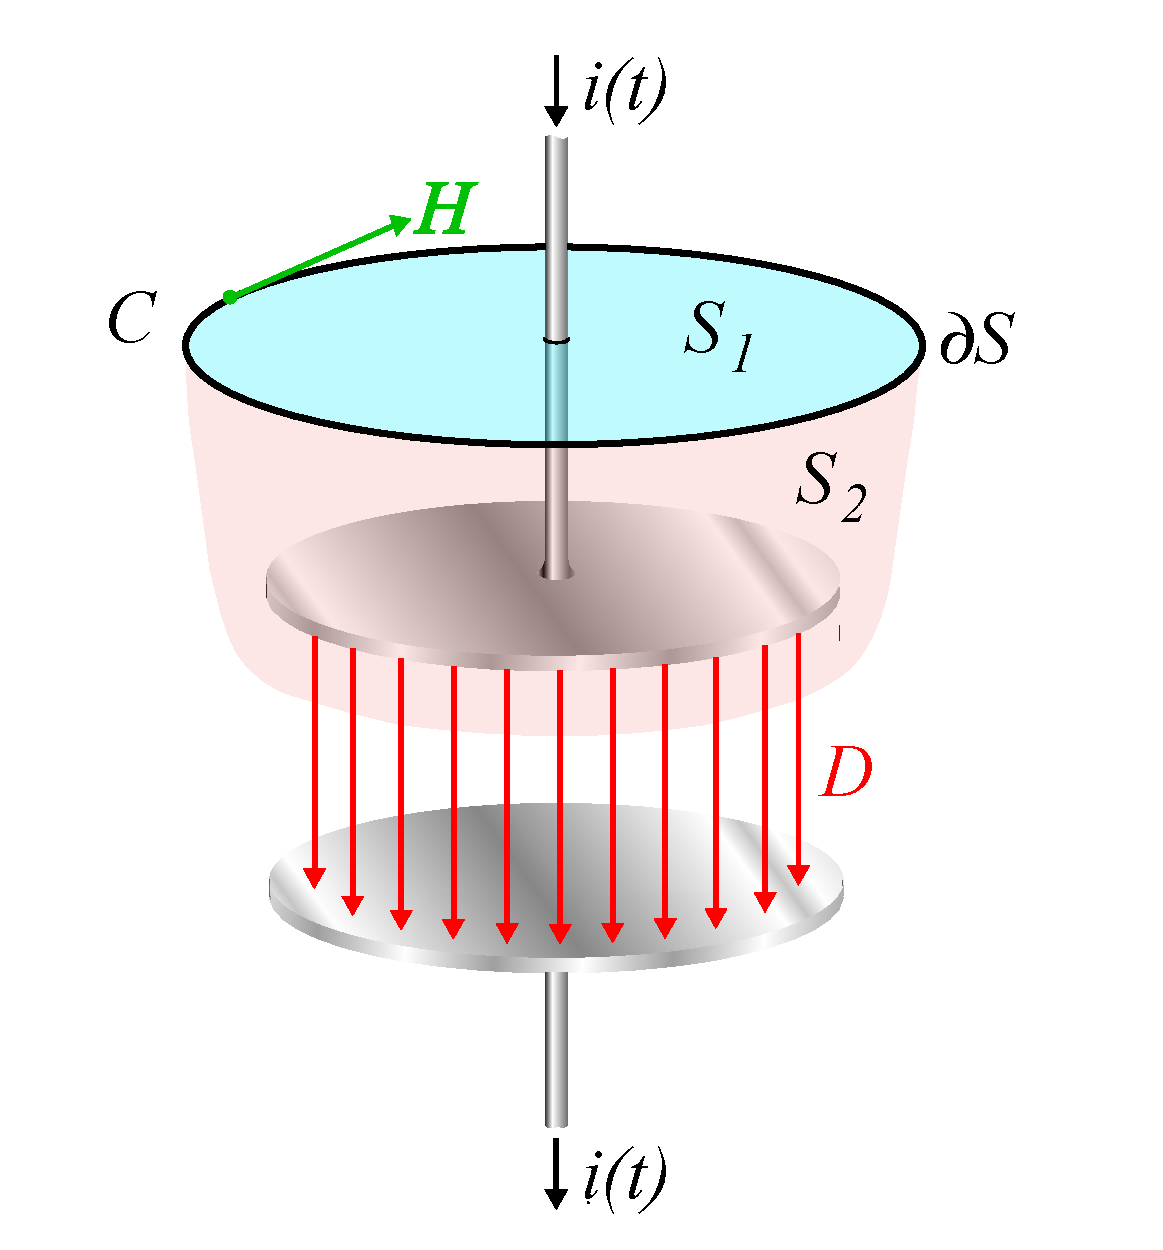
\includegraphics[width=7cm]{image/Displacement_current_in_capacitor.pdf}
\end{Figure}
在$S_1$上适用安培环路定律,由于通过$S_1$的电流是$i(t)$
\begin{Equation}&[3]
    \Ilot[C]\vb*{H}\cdot\dd{\vb*{l}}=i(t)
\end{Equation}
在$S_2$上适用安培环路定律,由于通过$S_2$的电流是$0$
\begin{Equation}
    \Ilot[C]\vb*{H}\cdot\dd{\vb*{l}}=0
\end{Equation}
但是,磁场强度$\vb*{H}$在同一闭合曲线$C$上的环流不可能同时为$i(t)$和$0$,产生矛盾。针对该问题,麦克斯韦认为,电容器的两个极板间必然存在另一种形式的电流。电容器极板间电荷分布随着时间变化,电容极板间形成时变电场,麦克斯韦位移电流假设就在于,他认为,\empx{时变电场也是电流},称为\uwave{位移电流}(Displacement Current),区别于\uwave{传导电流}(Conduction Current)。

将\fancyref{ppt:电介质中的高斯定律}代入\fancyref{eqt:电流连续性方程}
\begin{Equation}&[4]
    \div\vb*{J}=-\pdv{\rho}{t}=-\pdv{t}\qty(\div\vb*{D})=-\div\pdv{\vb*{D}}{t}
\end{Equation}
即
\begin{Equation}&[5]
    \div(\vb*{J}+\pdv{\vb*{D}}{t})=0
\end{Equation}
这里$\pdv*{\vb*{D}}{t}$是电位移随时间的变化率,称为位移电流密度,记作$\vb*{J}_\text{d}$。

这里\xrefpeq{5}重新诠释了电流连续性方程,在过去的版本中,电流场只有在恒定条件下才是连续的,电流在电荷密度发生变化处产生源和汇,在新的观点下,我们认为电流应当要同时包含传导电流和位移电流,这样即便在时变电磁场的情形下,电流也都是连续的了。如果回到前面电容的例子,在导线上电流以运动电荷的传导电流的形态进行传输,在电容中电流以时变电场的位移电流的形态进行传输,两者大小相等,形成连续的电流,尽管电容中没有任何导线。

而位移电流和传导电流一样,均需要产生磁场,因而安培环路定律需要修正为
\begin{Equation}&[6]
    \curl\vb*{H}=\vb*{J}+\pdv{\vb*{D}}{t}
\end{Equation}
现在两端取散度就不会再出现任何矛盾了,考虑到\xrefpeq{5}的结果。

而如果我们抛开位移电流这些表象,其实\xrefpeq{6}就告诉我们,时变电场产生磁场。
\begin{BoxProperty}[时变电场产生涡旋磁场]
    时变电场,是磁场的正涡旋源
    \begin{Equation}
        \grad\times\vb*{H}=\vb*{J}+\pdv{\vb*{D}}{t}
    \end{Equation}
\end{BoxProperty}

这里我们或许会想,为什么“变化的电场”的效果可以等效为位移电流,而“变化的磁场”的效果则不能等效为某种古怪的电荷?这种不对称性来自哪里?关键是在于,变化的电场和磁场总是充当对方的涡旋源,但在静电学和静磁学理论中,电场的源是电荷,磁场的源是电流
\begin{itemize}
    \item 电流是磁场的涡旋源,因此变化电场产生的磁场的涡旋源可以视作某种电流。
    \item 电荷是电场的通量源,因此变化磁场产生的电场的涡旋源不能视作某种电荷。
\end{itemize}
\section{麦克斯韦方程组}
麦克斯韦电磁理论的基础是本章\xref{sec:真空中静电场的基本规律}、\xref{sec:真空中静磁场的基本规律}、\xref{sec:电磁感应和位移电流}中提到的电磁学三大实验定律:库伦定律、安培力定律、法拉第电磁感应定律。这三个实验定律都是在各自的特定条件下总结出来的,而麦克斯韦在前人得到的实验结果的基础上,通过科学的假设和符合逻辑的分析,最终在1864年,归纳总结出了\uwave{麦克斯韦方程组}(Maxwell's Equations),统一了电磁理论。\cite{W3}

\begin{Figure}[麦克斯韦]
    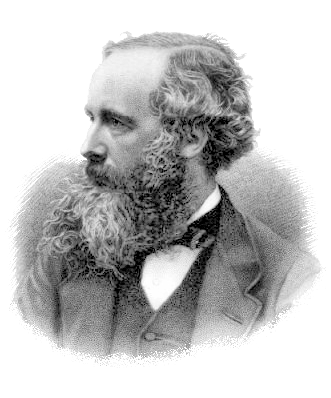
\includegraphics[width=4.4cm]{image/James_Clerk_Maxwell.png}
\end{Figure}

\subsection{麦克斯韦方程组}
麦克斯韦方程组实质上,就是对前面五个小节结论的汇总,它完整的表述了电磁场的性质。\footnote{记得高二那年初次听闻麦克斯韦方程组,那时,虽不知其意,但仍被其优美和简洁所震撼。时至今日,已经过去了整整三年,我想这一天对我来说会是一个值得纪念的日子,三年的等待,三年的准备,我终于看见了电磁波。—— 2023.03.24 写于钱伟长图书馆}
\begin{BoxEquation}[麦克斯韦方程组]
    麦克斯韦方程组描述了电磁场的基本形状,包含以下四个方程
    \begin{Gather}[10pt]
        \curl\vb*{H}=\vb*{J}+\pdv{\vb*{D}}{t}\xlabelpeq{磁场旋度}\\
        \curl\vb*{E}=-\pdv{\vb*{B}}{t}\xlabelpeq{电场旋度}\\
        \div\vb*{B}=0\xlabelpeq{磁场散度}\\
        \div\vb*{D}=\rho\xlabelpeq{电场散度}
    \end{Gather}
    除此之外,另有三组本构关系作为电磁场的辅助方程
    \begin{Equation}
        \vb*{D}=\varepsilon\vb*{E}\qquad
        \vb*{B}=\mu\vb*{H}\qquad
        \vb*{J}=\sigma\vb*{E}
    \end{Equation}
\end{BoxEquation}

麦克斯韦方程组,从内容上看,其实就是阐述了以下四个事实
\begin{center}
    \ttfamily

    电荷是电场的通量源,电流是磁场的涡旋源

    变化的磁场是电场的负涡旋源,变化的电场是磁场的正涡旋源
\end{center}
麦克斯韦的方程组的四个方程,依次从旋度和散度说明了磁场和电场的性质
\begin{enumerate}
    \item 磁场的旋度,源自变化的电场和传导电流。
    \item 电场的旋度,源自变化的磁场。
    \item 磁场的散度,始终为零。
    \item 电场的散度,源自电荷。
\end{enumerate}
我们可能会注意到,尽管麦克斯韦方程组的数学形式非常优美,但是好像总有一些不对称,这种不对称性其实来自,我们只有“电荷和电流”,并没有所谓“磁荷和磁流”,假如磁荷真的存在的话\cite{W3},那么$\div\vb*{B}$即为磁荷,而$\curl\vb*{E}$中亦要补充磁流项,这样方程就完全对应了。\footnote{虽然这样说,但或许正是电场和磁场间,以及千千万万更多事物间的不对称性,才有了我们这个精彩而灵动的世界。}

麦克斯韦方程组亦有积分形式,列写如下
\begin{Gather}[12pt]
    \Ilot[C]\vb*{H}\cdot\dd{\vb*{l}}=\Isnt[S]\qty(\vb*{J}+\pdv{\vb*{D}}{t})\cdot\dd{\vb*{S}}\\
    \Ilot[C]\vb*{E}\cdot\dd{\vb*{l}}=-\Isnt[S]\pdv{\vb*{B}}{t}\cdot\dd{\vb*{S}}\\
    \Isot[S]\vb*{B}\cdot\dd{\vb*{S}}=0\\
    \Isot[S]\vb*{D}\cdot\dd{\vb*{S}}=\Itnt[V]\rho\dd{V}
\end{Gather}
但在实际应用中,我们还是会更多的使用麦克斯韦方程的微分形式而不是积分形式。


实际上,在时变条件下,麦克斯韦方程组的四个方程之间并不是完全独立的,我们可以由它的两个旋度方程部分推导出两个散度方程,至多允许与原有的两个散度方程相差一个常数。\footnote{所以,实际上还是不独立的?或者说,两个散度方程的意义就是明确这个常数的值?}

\paragraph{由电场旋度方程推导磁场散度方程}
我们在电场的旋度方程\xrefpeq{电场旋度}两端取散度
\begin{Equation}
    \div(\curl\vb*{E})=-\pdv{t}(\div\vb*{B})
\end{Equation}
由于旋度的散度为零,这里$\div(\curl\vb*{E})=0$
\begin{Equation}
    \pdv{t}(\div\vb*{B})=0
\end{Equation}
这表明$\div\vb*{B}=$是常数,这与磁场散度方程的$\div\vb*{B}=0$至多相差一个常数。

\paragraph{由磁场旋度方程推导电场散度方程}
我们在磁场的旋度方程\xrefpeq{磁场旋度}两端取散度
\begin{Equation}
    \div(\curl\vb*{H})=\div\vb*{J}+\pdv{t}(\div\vb*{D})
\end{Equation}
由于旋度的散度为零,这里$\div(\curl\vb*{H})=0$
\begin{Equation}
    \pdv{t}(\div\vb*{D})+\div\vb*{J}=0
\end{Equation}
代入\fancyref{eqt:电流连续性方程},即$\div\vb*{J}=-\pdv*{\rho}{t}$
\begin{Equation}
    \pdv{t}(\div\vb*{D}-\rho)=0
\end{Equation}
这表明$\div\vb*{D}-\rho$是常数,这与电场散度方程\xrefpeq{电场散度}的$\div\vb*{D}=\rho$至多相差一个常数。

\subsection{电准静态电磁场}
在麦克斯韦方程组中,若$\pdv*{\vb*{B}}{t}$项可以忽略,即感应电场远小于库伦电场,例如电容器中的电磁场,则可以得到\uwave{电准静态电磁场},电准静态下,尽管$\vb*{E},\vb*{D}$时变,但却适用静电场的规律。
\begin{BoxEquation}[电准静态电磁场]
    电准静态电磁场,是指$\pdv*{\vb*{B}}{t}$项可以忽略,此时麦克斯韦方程组
    \begin{Gather}[10pt]
        \curl\vb*{H}=\vb*{J}+\pdv{\vb*{D}}{t}\\
        \curl\vb*{E}=0\\
        \div\vb*{B}=0\\
        \div\vb*{D}=\rho
    \end{Gather}
\end{BoxEquation}

\subsection{磁准静态电磁场}
在麦克斯韦方程组中,若$\pdv*{\vb*{D}}{t}$项可以忽略,即位移电流远小于传导电流,例如电感器中的电磁场,则可以得到\uwave{磁准静态电磁场},磁准静态下,尽管$\vb*{B},\vb*{H}$时变,但却适用静磁场的规律。
\begin{BoxEquation}[磁准静态电磁场]
    磁准静态电磁场,是指$\pdv*{\vb*{D}}{t}$项可以忽略,此时麦克斯韦方程组
    \begin{Gather}[10pt]
        \curl\vb*{H}=\vb*{J}\\
        \curl\vb*{E}=-\pdv{\vb*{B}}{t}\\
        \div\vb*{B}=0\\
        \div\vb*{D}=\rho
    \end{Gather}
\end{BoxEquation}
\section{电磁场的边界条件}
在解决实际的电磁场工程问题中,通常要设计到不同电磁参数的物质所构成的相邻区域。由于电磁参数在物质分界面上发生了变化,导致电磁场矢量也会随之发生突变,使\xref{sec:麦克斯韦方程组}中的麦克斯韦方程的微分形式在分界面上失去意义。这种情况下,为了求解各个区域中的电磁场问题,必须要知道在两种物质分界面两侧的电磁场量间的关系,我们称为\uwave{电磁场的边界条件}。

边界条件在求解电磁问题的过程中占据非常重要的地位,这是因为只有使得麦克斯韦方程组的通解适合于某个包含给定的区域及其边界条件,这个解,才是有实际意义的唯一解。

边界条件如何求呢?关键在于利用麦克斯韦方程组的积分形式,因为积分形式的麦克斯韦方程组不受场量连续与否的影响,在边界上也是成立的。本节就将以这种方式导出边界条件。

在接下来两个小节中,我们均以$\vb*{e}_\text{n}$表示分界面上,由介质1指向介质2的法向矢量。

\subsection{切向边界条件}
\begin{BoxFormula}[磁场强度的边界条件]
    磁场强度的边界条件满足
    \begin{Equation}
        \vb*{e}_\text{n}\times(\vb*{H}_1-\vb*{H}_2)=\vb*{J}_{S}
    \end{Equation}
    这表明,磁场强度的切向分量在分界面发生跃变,跃变量为面电流密度。
\end{BoxFormula}
\begin{Proof}
    如\xref{fig:介质分界面上的小矩形回路}所示,设想,我们现在考察介质分界面上的某一点$P$处的情况,我们在点$P$的周围取一个小矩形回路$ABCD$,设其所围面积是$\delt{S}$。矩形回路$AB$和$CD$两条边分别位于分界面的两侧并与之平行,其长度$AB=CD=\delt{l}$很小,其间距$BC=DA=\delt{h}\to 0$趋于零。
    \begin{Figure}[介质分界面上的小矩形回路]
        \includegraphics[scale=0.9]{build/Chapter02G_01.fig.pdf}
    \end{Figure}
    这里我们主要涉及到三个单位矢量
    \begin{itemize}
        \item 单位矢量$\vb*{e}_\text{n}$表示两种介质的边界曲面上的法向矢量。
        \item 单位矢量$\vb*{e}_\text{p}$表示矩形区域面积$\delt{S}$的法向矢量(图中未绘出)。
        \item 单位矢量$\vb*{e}_\text{t}$表示沿矩形$AB$方向上的单位矢量。
    \end{itemize}
    第一步,我们运用\fancyref{eqt:麦克斯韦方程组的积分形式}
    \begin{Equation}&[1]
        \Ilot[C]\vb*{H}\cdot\dd{\vb*{l}}=\Isnt[\delt{S}]\vb*{J}\cdot\dd{\vb*{S}}+\Isnt[\delt{S}]\pdv{\vb*{D}}{t}\cdot\dd{\vb*{S}}
    \end{Equation}
    这里$C$就是小矩形回路$ABCD$,我们前面提到过,我们要令$\delt{h}\to 0$。

    由于电位移$\vb*{D}$是连续变化的,因此$\pdv*{\vb*{D}}{t}$应当是有限值,故
    \begin{Equation}&[2]
        \Lim[\delt{h}\to 0]\Isnt[\delt{S}]\pdv{\vb*{D}}{t}\cdot\dd{\vb*{S}}=0
    \end{Equation}
    由于当$\delt{h}\to 0$时,真正对$\delt{S}$的电流密度通量有贡献的必然是分界面上的面电流$\vb*{J}_{S}$,故
    \begin{Equation}&[3]
        \Lim[\delt{h}\to 0]\Isnt[\delt{S}]\vb*{J}\cdot\dd{\vb*{S}}=\Ilnt[\delt{l}]\vb*{J}_S\cdot\vb*{e}_\text{p}\dd{l}
    \end{Equation}
    这样一来,将\xrefpeq{2}和\xrefpeq{3}代回\xrefpeq{1}
    \begin{Equation}&[4]
        \Lim[\delt{h}\to 0]\Ilot[C]\vb*{H}\cdot\dd{\vb*{l}}=\Ilnt[\delt{l}]\vb*{J}_S\cdot\vb*{e}_\text{p}\dd{l}
    \end{Equation}
    第二步,我们将$\vb*{H}$沿$C$的积分拆为四段
    \begin{Equation}&[5]
        \Ilot[C]\vb*{H}\cdot\dd{\vb*{l}}=\Ilnt[AB]\vb*{H}\cdot\dd{\vb*{l}}
        +\Ilnt[BC]\vb*{H}\cdot\dd{\vb*{l}}
        +\Ilnt[CD]\vb*{H}\cdot\dd{\vb*{l}}
        +\Ilnt[DA]\vb*{H}\cdot\dd{\vb*{l}}
    \end{Equation}
    由于磁场强度$\vb*{H}$应当是有限值,故
    \begin{Equation}&[6]
        \Lim[\delt{h}\to 0]\qty[
            \Ilnt[BC]\vb*{H}\cdot\dd{\vb*{l}}+
            \Ilnt[DA]\vb*{H}\cdot\dd{\vb*{l}}
        ]=0
    \end{Equation}
    而同时,随着$\delt{h}\to 0$,路径$AB,CD$都缩到同一条路径$\delt{l}$上,但在边界两侧沿相反方向
    \begin{Equation}&[7]
        \Lim[\delt{h}\to 0]\qty[
            \Ilnt[AB]\vb*{H}\cdot\dd{\vb*{l}}+
            \Ilnt[CD]\vb*{H}\cdot\dd{\vb*{l}}
        ]=\Ilnt[\delt{l}](\vb*{H}_1-\vb*{H}_2)\cdot\vb*{e}_\text{t}\dd{l}
    \end{Equation}
    这样一来,将\xrefpeq{6}和\xrefpeq{7}代入\xrefpeq{5}
    \begin{Equation}&[8]
        \Lim[\delt{h}\to 0]\Ilot[c]\vb*{H}\cdot\dd{\vb*{l}}=\Ilnt[\delt{l}](\vb*{H}_1-\vb*{H}_2)\cdot\vb*{e}_\text{t}\dd{l}
    \end{Equation}
    由此,联立\xrefpeq{4}和\xrefpeq{8},得到
    \begin{Equation}&[9]
        \Ilnt[\delt{l}]\vb*{J}_{S}\cdot\vb*{e}_\text{p}\dd{l}=\Ilnt[\delt{l}](\vb*{H}_1-\vb*{H}_2)\cdot\vb*{e}_\text{t}\dd{l}
    \end{Equation}
    由于$\delt{l}$很小时,可以认为$\vb*{H}_1,\vb*{H}_2,\vb*{J}_S$都是均匀的,故
    \begin{Equation}&[10]
        \vb*{J}_{S}\cdot\vb*{e}_\text{p}\delt{l}=(\vb*{H}_1-\vb*{H}_2)\cdot\vb*{e}_\text{t}\delt{l}
    \end{Equation}
    两端约去$\delt{l}$
    \begin{Equation}&[11]
        \vb*{J}_{S}\cdot\vb*{e}_\text{p}=(\vb*{H}_1-\vb*{H}_2)\cdot\vb*{e}_\text{t}
    \end{Equation}
    由于$\vb*{e}_\text{t}=\vb*{e}_\text{p}\times\vb*{e}_\text{n}$,代入\xrefpeq{11}右端,并使用\fancyref{fml:标量三重积的轮换对称性}
    \begin{Equation}&[12]
        \qquad\qquad\quad
        (\vb*{H}_1-\vb*{H}_2)\cdot\vb*{e}_\text{t}=(\vb*{H}_1-\vb*{H}_2)\cdot(\vb*{e}_\text{p}\times\vb*{e}_\text{n})=\qty[\vb*{e}_\text{n}\times(\vb*{H}_1-\vb*{H}_2)]\cdot\vb*{e}_\text{p}
        \qquad\qquad\quad
    \end{Equation}
    将\xrefpeq{12}代入\xrefpeq{11}
    \begin{Equation}&[13]
        \vb*{J}_{S}\cdot\vb*{e}_\text{p}=\qty[\vb*{e}_\text{n}\times(\vb*{H}_1-\vb*{H}_2)]\cdot\vb*{e}_\text{p}
    \end{Equation}
    约去$\vb*{e}_\text{p}$即得
    \begin{Equation}*
        \vb*{e}_\text{n}\times(\vb*{H}_1-\vb*{H}_2)=\vb*{J}_{S}\qedhere
    \end{Equation}
\end{Proof}
% 由此可见,分界面上存在自由面电流时,分界面两侧的磁场强度矢量$\vb*{H}$的切向分量是不连续的。这是因为电流是磁场强度$\vb*{H}$的涡旋源,在分界面上的面电流在分界面两侧产生的磁场强度矢量,在切向是相反的,这就导致了$\vb*{H}$在切向上的跃变。

\begin{BoxFormula}[电场强度的边界条件]
    电场强度的边界条件满足
    \begin{Equation}
        \vb*{e}_\text{n}\times(\vb*{E}_1-\vb*{E}_2)=\vb*{0}
    \end{Equation}
    这表明,电场强度的切向分量在分界面是连续的。
\end{BoxFormula}

\begin{Proof}
    如\xref{fig:介质分界面上的小矩形回路},只不过图中的磁场强度$\vb*{H}_1,\vb*{H}_2$应当改换为电场强度$\vb*{E}_1,\vb*{E}_2$。

    第一步,我们运用\fancyref{eqt:麦克斯韦方程组的积分形式}
    \begin{Equation}&[1]
        \Ilot[C]\vb*{E}\cdot\dd{\vb*{l}}=\Isnt[S]\pdv{\vb*{B}}{t}\cdot\dd{\vb*{S}}
    \end{Equation}

    由于磁感应强度$\vb*{B}$是连续变化的,因此$\pdv*{B}{t}$应当是有限值,故
    \begin{Equation}&[2]
        \Lim[\delt{h}\to 0]\Isnt[S]\pdv{\vb*{B}}{t}\cdot\dd{\vb*{S}}=0
    \end{Equation}
    因而
    \begin{Equation}&[3]
        \Lim[\delt{h}\to 0]\Ilot[C]\vb*{E}\cdot\dd{\vb*{l}}=0
    \end{Equation}
    第二步,根据前面的经验
    \begin{Equation}&[4]
        \Lim[\delt{h}\to 0]\Ilot[C]\vb*{E}\cdot\dd{\vb*{l}}=\Ilnt[\delt{l}](\vb*{E}_1-\vb*{E}_2)\cdot\vb*{e}_\text{t}\dd{l}
    \end{Equation}
    联立\xrefpeq{3}和\xrefpeq{4},再效仿前面的转化方法,最终得到
    \begin{Equation}*
        \vb*{e}_\text{n}\times(\vb*{E}_1-\vb*{E}_2)=\vb*{0}\qedhere
    \end{Equation}
\end{Proof}

\subsection{法向边界条件}
\begin{BoxFormula}[电位移矢量的边界条件]
    电位移矢量的边界条件满足
    \begin{Equation}
        \vb*{e}_\text{n}\cdot(\vb*{D}_1-\vb*{D}_2)=\rho_S
    \end{Equation}
    这表明,电位移矢量在法向分量在分界面发生跃变,跃变量为面电荷密度。
\end{BoxFormula}

\begin{Proof}
    如\xref{fig:介质分界面上的小圆柱形闭合曲面}所示,设想,我们现在考察介质分界面上的某一点$P$处的情况,我们在点$P$的周围取一个底面积$\delt{S}$很小,高$\delt{h}\to 0$的小圆柱形闭合曲面,上下底面平行位于分界面两侧。
    \begin{Figure}[介质分界面上的小圆柱形闭合曲面]
        \includegraphics[scale=0.9]{build/Chapter02G_02.fig.pdf}
    \end{Figure}

    第一步,我们运用\fancyref{eqt:麦克斯韦方程组的积分形式}
    \begin{Equation}&[1]
        \Isot[S]\vb*{D}\cdot\dd{\vb*{S}}=\Itnt[V]\rho\dd{V}
    \end{Equation}
    这里$S$就是小圆柱形闭合曲面,而$V$是该闭合曲面包围的空间区域,我们要令$\delt{h}\to 0$。

    由于当$\delt{h}\to 0$时,真正对$V$中的电荷量有贡献的必然是分界面上的面电荷$\rho_S$,故
    \begin{Equation}&[2]
        \Lim[\delt{h}\to 0]\Itnt[V]\rho\dd{V}=\Isnt[\delt{S}]\rho_S\dd{S}
    \end{Equation}
    这样一来,将\xrefpeq{2}代入\xrefpeq{1}
    \begin{Equation}&[3]
        \Lim[\delt{h}\to 0]\Isot[S]\vb*{D}\cdot\dd{\vb*{S}}=\Isnt[\delt{S}]\rho_S\dd{S}
    \end{Equation}
    第二步,我们将$\vb*{D}$在闭合圆柱面上的积分拆分为底面和侧面
    \begin{Equation}&[4]
        \Isot[S]\vb*{D}\cdot\dd\vb*{S}=
        \Isnt[\text{上底面}]\vb*{D}\cdot\dd{\vb*{S}}+
        \Isnt[\text{下底面}]\vb*{D}\cdot\dd{\vb*{S}}+
        \Isnt[\text{侧面}]\vb*{D}\cdot\dd{\vb*{S}}
    \end{Equation}
    由于电位移矢量$\vb*{D}$应当是有限值,故
    \begin{Equation}&[5]
        \Lim[\delt{h}\to 0]\Isnt[\text{侧面}]\vb*{D}\cdot\dd{\vb*{S}}=0
    \end{Equation}
    而同时,随着$\delt{h}\to 0$,上下底面都缩到$\delt{S}$上,但两者朝向相反
    \begin{Equation}&[6]
        \Lim[\delt{h}\to 0]\qty[\Isnt[\text{上底面}]\vb*{D}\cdot\dd{\vb*{S}}+
        \Isnt[\text{下底面}]\vb*{D}\cdot\dd{\vb*{S}}]=\Isnt[\delt{S}](\vb*{D}_1-\vb*{D}_2)\cdot\vb*{e}_\text{n}\dd{S}\hspace*{-0.1cm}
    \end{Equation}
    这样一来,将\xrefpeq{5}和\xrefpeq{6}代入\xrefpeq{4}
    \begin{Equation}&[7]
        \Lim[\delt{h}\to 0]\Isot[S]\vb*{D}\cdot\dd{\vb*{S}}=\Isnt[\delt{S}](\vb*{D}_1-\vb*{D}_2)\cdot\vb*{e}_\text{n}\dd{S}
    \end{Equation}
    由此,联立\xrefpeq{3}和\xrefpeq{7},得到
    \begin{Equation}
        \Isnt[\delt{S}]\rho_S\dd{S}=\Isnt[\delt{S}](\vb*{D}_1-\vb*{D}_2)\cdot\vb*{e}_\text{n}\dd{S}
    \end{Equation}
    即
    \begin{Equation}*
        \vb*{e}_\text{n}\cdot(\vb*{D}_1-\vb*{D}_2)=\rho_S\qedhere
    \end{Equation}
\end{Proof}

\begin{BoxFormula}[磁感应强度的边界条件]
    磁感应强度的边界条件满足
    \begin{Equation}
        e_\text{n}\cdot(\vb*{B}_1-\vb*{B}_2)=0
    \end{Equation}
    这表明,磁感应强度的法向分量在分界面是连续的。
\end{BoxFormula}

\begin{Proof}
    如\xref{fig:介质分界面上的小圆柱形闭合曲面},只不过图中的电位移矢量$\vb*{D}_1,\vb*{D}_2$应当改换为磁感应强度$\vb*{B}_1,\vb*{B}_2$。

    第一步,我们应用\fancyref{eqt:麦克斯韦方程组的积分形式}
    \begin{Equation}&[1]
        \Isot[S]\vb*{B}\cdot\dd{\vb*{S}}=0
    \end{Equation}
    因而,很显然的
    \begin{Equation}&[2]
        \Lim[\delt{h}\to 0]\Isot[S]\vb*{B}\cdot\dd{\vb*{S}}=0
    \end{Equation}
    第二步,根据前面的经验
    \begin{Equation}&[3]
        \Lim[\delt{h}\to 0]\Isot[S]\vb*{B}\cdot\dd{\vb*{S}}=\Isnt[\delt{S}](\vb*{B}_1-\vb*{B}_2)\cdot\vb*{e}_\text{n}\dd{S}
    \end{Equation}
    联立\xrefpeq{2}和\xrefpeq{3},得到
    \begin{Equation}*
        e_\text{n}\cdot(\vb*{B}_1-\vb*{B}_2)=0\qedhere
    \end{Equation}
\end{Proof}

在此,让我们来总结一下四个电磁场矢量的边界条件
\begin{itemize}
    \item \xref{fml:磁场强度的边界条件}指出,矢量$\vb*{H}$的切向分量在边界不连续,发生面电流密度的跃变。
    \item \xref{fml:电场强度的边界条件}指出,矢量$\vb*{E}$的切向分量在边界连续。
    \item \xref{fml:磁感应强度的边界条件}指出,矢量$\vb*{B}$的法向分量在边界连续。
    \item \xref{fml:电位移矢量的边界条件}指出,矢量$\vb*{D}$的法向分量在边界不连续,发生面电荷密度的跃变。
\end{itemize}
在这里,一个有趣的问题是,为什么面电流和面电荷导致的跃变分别是切向和法向?
\begin{itemize}
    \item 面电流密度是$\vb*{H}$的涡旋源,涡旋源在分界面两侧产生的场,切向相反。
    \item 面电荷密度是$\vb*{D}$的通量源,通量源在分界面两侧产生的场,法向相反。
\end{itemize}
还有一个值得注意的问题是,由于
\begin{Equation}
    \vb*{J}_{S}=\Lim[\delt{h}\to 0]\vb*{J}\delt{h}=\Lim[\delt{h}\to 0]\sigma\vb*{E}\delt{h}
\end{Equation}
由于电场强度$\vb*{E}$为有限值,而$\delt{h}\to 0$,因此,面电流密度$\vb*{J}_{S}$若要有非零值,就必须要使得电导率$\sigma$为无穷大,换言之,电导率有限的介质中,矢量$\vb*{H}$的切向分量在边界将是连续的。

\subsection{理想导体的边界条件}
\uwave{理想导体},就是指电导率很高,可以近似为无穷大的物质,例如银、铜、铝等金属
\begin{itemize}
    \item 理想导体的电导率为无穷大,因而边界面上可以存在面电流分布。
    \item 理想导体内部存在自由电荷,因而边界面上可以存在面电荷分布。
\end{itemize}
\begin{BoxFormula}[理想导体的边界条件]
    理想导体的边界条件满足
    \begin{Gather}[4pt]
        \vb*{e}_\text{n}\times\vb*{H}=\vb*{J}_S\\
        \vb*{e}_\text{n}\times\vb*{E}=\vb*{0}\\
        \vb*{e}_\text{n}\cdot\vb*{B}=0\\
        \vb*{e}_\text{n}\cdot\vb*{D}=\rho_S
    \end{Gather}
\end{BoxFormula}
理想导体内部还有许多重要的性质,由于理想导体的电导率$\sigma$为无穷大,根据$\vb*{J}=\sigma\vb*{E}$,这表明电场强度$\vb*{E}$应恒为零,否则将出现无限大的电流分布,因此,\empx{理想导体中不存在电场}。而进一步,我们由电磁感应原理$\curl\vb*{E}=-\pdv*{\vb*{B}}{t}=\vb*{0}$可知,\empx{理想导体中亦不存在时变磁场}。

\subsection{理想介质的边界条件}
理想介质,就是指电导率很低,可以近似为零的物质,例如聚苯乙烯、陶瓷
\begin{itemize}
    \item 理想介质的电导率为零,因而边界面上不存在面电流分布。
    \item 理想介质内部没有自由电荷,因而边界面上也不可能存在自由面电荷分布。
\end{itemize}
理想介质边界面上可以有束缚面电荷分布,但这不是$\div\vb*{D}=\rho$所关心的。
\begin{BoxFormula}[理想导体的边界条件]*
    理想导体的边界条件满足
    \begin{Gather}[4pt]
        \vb*{e}_\text{n}\times(\vb*{H}_1-\vb*{H}_2)=\vb*{0}\\
        \vb*{e}_\text{n}\times(\vb*{E}_1-\vb*{E}_2)=\vb*{0}\\
        \vb*{e}_\text{n}\cdot(\vb*{B}_1-\vb*{B}_2)=0\\
        \vb*{e}_\text{n}\cdot(\vb*{D}_1-\vb*{D}_2)=0
    \end{Gather}
\end{BoxFormula}